% Autor: Leonhard Segger, Jannik Tim Zarnitz
% Datum: 2017-10-30
\documentclass[
% Papierformat
a4paper,
% Schriftgröße (beliebige Größen mit „fontsize=Xpt“)
12pt,
% Schreibt die Papiergröße korrekt ins Ausgabedokument
pagesize,
% Sprache für z.B. Babel
ngerman
]{scrartcl}

% Achtung: Die Reihenfolge der Pakete kann (leider) wichtig sein!
% Insbesondere sollten (so wie hier) babel, fontenc und inputenc (in dieser
% Reihenfolge) als Erstes und hyperref und cleveref (Reihenfolge auch hier
% beachten) als Letztes geladen werden!

\usepackage{tikz}
\usetikzlibrary{calc,patterns,angles,quotes} % loads some tikz extensions\usepackage{tikz}
\usetikzlibrary{babel}

% Silbentrennung etc.; Sprache wird durch Option bei \documentclass festgelegt
\usepackage{babel}
% Verwendung der Zeichentabelle T1 (Sonderzeichen etc.)
\usepackage[T1]{fontenc}
% Legt die Zeichenkodierung der Eingabedatei fest, z.B. UTF-8
\usepackage[utf8]{inputenc}
% Schriftart
\usepackage{lmodern}
% Zusätzliche Sonderzeichen
\usepackage{textcomp}

% Mathepaket (intlimits: Grenzen über/unter Integralzeichen)
\usepackage[intlimits]{amsmath}
% Ermöglicht die Nutzung von \SI{Zahl}{Einheit} u.a.
\usepackage{siunitx}
% Zum flexiblen Einbinden von Grafiken (\includegraphics)
\usepackage{graphicx}
% Abbildungen im Fließtext
\usepackage{wrapfig}
% Abbildungen nebeneinander (subfigure, subtable)
\usepackage{subcaption}
% Funktionen für Anführungszeichen
\usepackage{csquotes}
\MakeOuterQuote{"}
% Zitieren, Bibliografie
\usepackage{biblatex}


% Zur Darstellung von Webadressen
\usepackage{url}
%chemische Formeln
\usepackage[version=4]{mhchem}
% siunitx: Deutsche Ausgabe, Messfehler getrennt mit ± ausgeben
\usepackage{floatrow}
\floatsetup[table]{capposition=top}
\usepackage{float}
% Verlinkt Textstellen im PDF-Dokument
\usepackage[unicode]{hyperref}
% "Schlaue" Referenzen (nach hyperref laden!)
\usepackage{cleveref}
\sisetup{
	locale=DE,
	separate-uncertainty
}
%\bibliography{6Mi_M3_29-11-2017_References}
%TODO anpassen

\begin{document}
	
	\begin{titlepage}
		\centering
		{\scshape\LARGE Protokoll zu \par}
		\vspace{1cm}
		{\scshape\huge Einführung in rechnergestütztes Experimentieren \par}
		\vspace{3cm}
		
		{\large Jannik Tim Zarnitz (E-Mail: j\_zarn02@wwu.de) \par}
		{\large Leonhard Segger (E-Mail: l\_segg03@wwu.de) \par}
		\vfill
		
		in der Woche 03.09.2018 bis 06.09.2018\par
		betreut von\par
		{\large Dr. Jürgen Berkemeier}
		
		\vfill
		
		{\large \today\par}
	\end{titlepage}
	\tableofcontents
	\newpage

	\section{Tag 1}
	
	\subsection{Aufbau einer Sinus- bzw. Bessel-Funktion} \label{sinusfkt}
	
	Zunächst soll unter Verwendung des graphischen Programmiersystems \glqq LabVIEW\grqq\ eine Sinus-Funktion realisiert werden. Mithilfe der von LabVIEW zur Verfügung gestellten numerischen Operationen, Konstanten und Schleifen lässt sich ein Programm schreiben, welches eine Sinusschwingung $u$ der Form
	
	\begin{equation} \label{u}
	u(A,f,t,\varphi) = A \cdot \sin(2\pi f t + \varphi) \ ,
	\end{equation}
	
	\noindent umsetzt. Wobei $A$ die Schwingungsamplitude, $f$ die Frequenz und $\varphi$ die Phasenverschiebung bilden. Außerdem ist jedes $t$ durch 
	
	\begin{equation} \label{t}
	t = \frac{i}{N}
	\end{equation}
	
	\noindent gegeben. $N$ ist dabei die Zahl der Stützstellen und zugleich die Anzahl der zu berechnenden Wertepaare. Der Index $i$ kann Werte im Bereich zwischen $0$ und $N$ annehmen. Der besagte Programmcode befindet sich im Blockdiagramm von LabVIEW und ist in \cref{sinusbesselprogrammcode} zu sehen. 
	
	\begin{figure}[H]
		\centering
		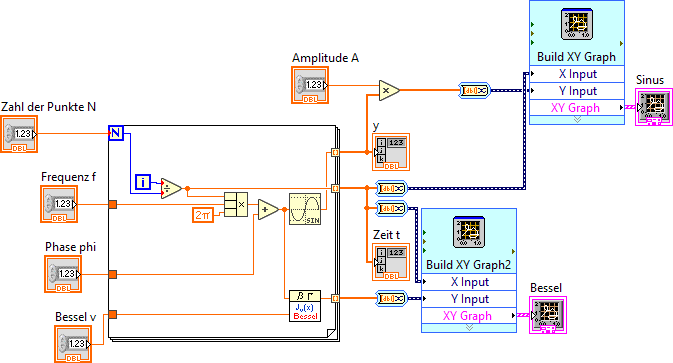
\includegraphics[width=1.0\textwidth]{EIRE2018Dateien/Tag1/sinusbessel-bilder/SinusBesseld}
		\caption{Die Abbildung zeigt ein LabVIEW-Blockdiagramm sowie den Aufbau des Programms zur Umsetzung einer Sinus- bzw. Bessel-Funktion. Die eigentliche Werte-Berechnung findet innerhalb der For-Schleife statt. Dazu werden feste, aber beliebige Fließkommazahlen für die Amplitude $A$, die Zahl der Punkte $N$, die Frequenz $f$, die Phase $\varphi$ und die Ordnung $\nu$ der Bessel-Funktion herangezogen. Die Ausgabe der Wertepaare erfolgt in Form zweier $X$-$Y$-Graphen sowie Arrays.}
		\label{sinusbesselprogrammcode}
	\end{figure}

	\noindent Das dazugehörige ausgegebene Frontpanel ist in \cref{sinusbesselausgabe} erkennbar. Die Gleitkommazahlen-Werte für $A$, $f$, $N$ und $\varphi$ sollen frei wählbar sein, zumal $u$ insbesondere von diesen abhängt. Das Programm ist daher so eingerichtet, dass auf der linken Seite des Frontpanels die entsprechenden Bedien- bzw. Eingabeelemente erscheinen. Unter gleichem Namen sind die jeweiligen Blockdiagrammobjekte im Programmcode zu finden. Im Zentrum des Programmcodes in \cref{sinusbesselprogrammcode} lässt sich eine For-Schleife erkennen. Gemäß \cref{u} sowie \cref{t} findet in dieser unter Verwendung des Laufindexes $i$ die tatsächliche Berechnung der $t$- und $u$-Werte statt. Die Blockdiagrammobjekte auf der rechten Seite des Programmcodes in \cref{sinusbesselprogrammcode} bilden die Anzeige- bzw. Ausgabeelemente des Frontpanels in \cref{sinusbesselausgabe}. Zum einen werden dabei zwei $N+1$ Einträge umfassende, eindimensionale Arrays angelegt, die jeweils alle $t$- sowie sämtliche $u$-Werte beinhalten und zum anderen wird ein $X$-$Y$-Diagramm erzeugt, in dem alle $u$-Werte gegen die entsprechenden $t$-Werte aufgetragen sind. Demnach befindet sich $t$ auf der $x$-Achse und $u$ auf der $y$-Achse. Um nun die Informationsübertragung zu bewerkstelligen, ist es notwendig im Programmcode vor den Anschlüssen der \glqq Build XY Graph\grqq -Kästen weitere Blockdiagrammobjekte hinzuzufügen, welche das Leitungssignal in ein für das Anzeigeelement ($X$-$Y$-Diagramm) passendes Eingangssignal umwandeln. Zumeist geschieht dies in LabVIEW automatisch und wird dann an der entsprechenden Stelle auf der Leitung mit einem kleinen, roten Punkt markiert.
			
	\begin{figure}[H]
		\centering
		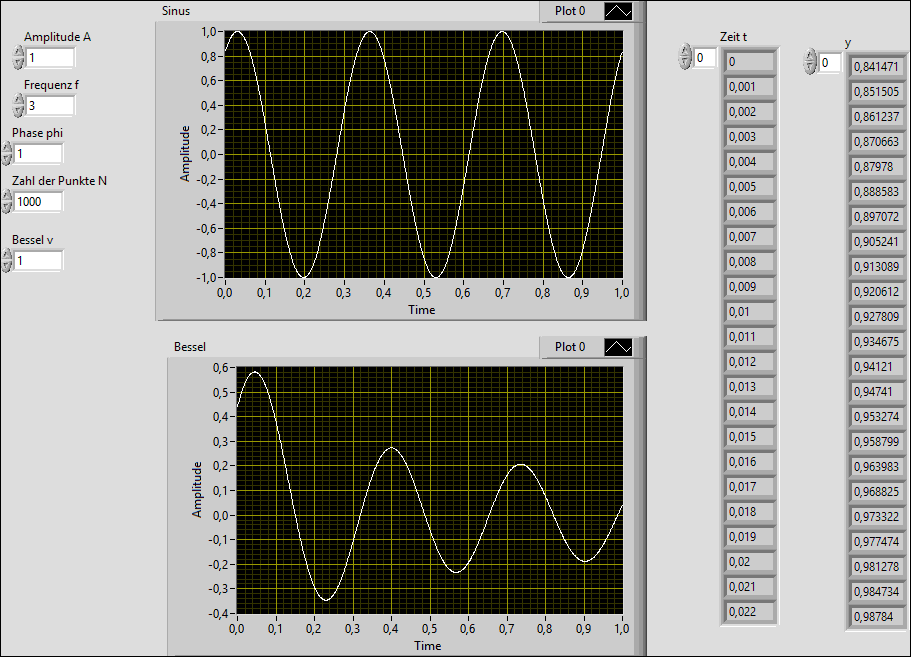
\includegraphics[width=1.0\textwidth]{EIRE2018Dateien/Tag1/sinusbessel-bilder/SinusBesselp}
		\caption{In dieser Abbildung ist das Frontpanel als Ausgabe und Benutzeroberfläche dargestellt.}
		\label{sinusbesselausgabe}
	\end{figure}

	\noindent Zusätzlich zur Sinus-Funktion wird eine Bessel-Funktion erster Gattung $J_{\nu}$ mit LabVIEW realisiert und ebenfalls in das Programm in \cref{sinusbesselprogrammcode} mit aufgenommen. Das entsprechende Blockdiagrammobjekt ist mit \glqq $J_{\nu}(x)$ Bessel\grqq\ gekennzeichnet. Die Bessel-Funktion besitzt die allgemeine Form
	
	\begin{equation}
	J_{\nu}(x) = \sum_{j=0}^{\infty}\frac{(-1)^j \cdot \left( \frac{x}{2}\right) ^{2j+\nu}}{j! \cdot \Gamma(\nu + j + 1)} \ .
	\end{equation}
	
	\noindent Wobei $\nu$ die Ordnung der Bessel-Funktion bildet, $\Gamma(\cdot)$ die Gamma-Funktion darstellt und $x$ auf Basis des Programmcodes in \cref{sinusbesselprogrammcode} als 
	
	\begin{equation}
	x := 2\pi f t + \varphi = \frac{2\pi f \cdot i}{N} + \varphi
	\end{equation}
	
	\noindent definiert ist. Der Fließkommazahlen-Wert für $\nu$ ist, ähnlich wie beim Sinus-Programm, über das entsprechende Bedienelement auf der linken Seite des Frontpanels einstellbar, was in \cref{sinusbesselausgabe} zu erkennen ist. Genauso wie beim Sinus-Programm findet die Berechnung der $x$- und $J_{\nu}(x)$-Werte innerhalb der For-Schleife statt. Die Werteausgabe erfolgt in Form eines $X$-$Y$-Diagramms, dessen Anzeigeelement im unteren Bereich der \cref{sinusbesselausgabe} ersichtlich ist und in dem $J_{\nu}(x)$ als Funktion von $x$ dargestellt ist. Zudem muss das Eingangssignal für das dazugehörige Blockdiagrammobjekt in \cref{sinusbesselprogrammcode} passend umgewandelt werden, so wie zuvor beim Sinus-Programm. 

	\begin{figure}[H]
		\centering
		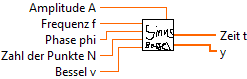
\includegraphics[width=1.0\textwidth]{EIRE2018Dateien/Tag1/sinusbessel-bilder/SinusBesselc}
		\caption{Die Abbildung zeigt das gestaltete Programm-Icon sowie die gesetzten Anschlussmöglichkeiten.}
		\label{sinusbesselicon}
	\end{figure}
	
	\noindent LabVIEW bietet die Möglichkeit ein bereits vorhandenes, selbst geschriebenes, funktionsfähiges Programm so zu bearbeiten, dass es für andere LabVIEW-Programme bzw. -Projekte als Blockdiagrammobjekt nutzbar wird. Dazu müssen zunächst die Anschlüsse festgelegt werden, sowohl die Eingänge als auch die Ausgänge. Allgemein kann es sich dabei um verschiedenste Arten von Ein-und Ausgangssignalen handeln. Bei der programmierten Sinus-Funktion verhält es sich demnach so, dass fünf Eingangs- und zwei Ausgangsanschlüsse generiert werden müssen, welche jeweils nur Gleitkommazahlen annehmen bzw. übergeben. Die Amplitude $A$, die Frequenz $f$, die Phasenverschiebung $\varphi$, die Anzahl der Punkte $N$ und die Ordnung $\nu$ der Bessel-Funktion bilden hierbei die Eingänge, die $t$-Werte sowie die $u$- bzw. $y$-Werte erscheinen über die beiden Ausgänge. Des Weiteren ist es in LabVIEW möglich das entsprechende Blockdiagrammobjekt-Icon des Programms zu gestalten. Das komplette Resultat ist in \cref{sinusbesselicon} dargestellt.
	
	\emph{Hinweis:} Aus der Betrachtung des Programmcodes in \cref{sinusbesselprogrammcode} geht hervor, dass das Blockdiagrammobjekt, welches das Array-Ausgabeelement des Frontpanels bildet und alle $u$-Werte abgreifen soll, inkorrekt eingefügt ist. Denn anstelle einer Implementierung nach der Multiplikation mit der Amplitude $A$, befindet sich das besagte Blockdiagrammobjekt davor. Sodass das Array lediglich die Werte des Ausdrucks
	
	\begin{equation}
	\sin(2\pi f t + \varphi)
	\end{equation}
	
	\noindent angibt, welche zwischen $-1$ und $1$ liegen. Da die Ausgabefunktion als Array einen erheblichen Einfluss auf das folgende Vorgehen hat, kann mit dem Sinus-Programm in dieser Form nicht weitergearbeitet werden. Im weiteren Verlauf der Projektbearbeitung ist der beschriebene Fehler allerdings behoben worden. Eine berichtigte, aktualisierte Version des Programms liegt an dieser Stelle jedoch nicht vor. 
	
	\subsection{Lissajous-Figuren}
	
	Im Folgenden sollen je nach Werteeinstellungen auf dem Anzeigeelement der Benutzeroberfläche verschiedene Lissajous-Figuren entstehen. Dies ist in \cref{lissajous} zu sehen. Die Basis für eine solche Lissajous-Figur bilden zwei verschiedene Sinusschwingungen, welche beide dieselbe Gestalt wie die \cref{u} besitzen:
	
	\begin{equation}
	u_1(A_1,f_1,t,\varphi_1) = A_1 \cdot \sin(2\pi f_1 t + \varphi_1) \ \ \ \textnormal{und} \ \ \ u_2(A_2,f_2,t,\varphi_2) = A_2 \cdot \sin(2\pi f_2 t + \varphi_2) \ ,
	\end{equation}
	
	\noindent mit den unterschiedlichen Amplituden $A_1$ und $A_2$, den Frequenzen $f_1$ und $f_2$ sowie den Phasenverschiebungen $\varphi_1$ und $\varphi_2$. Zudem bedarf es eines zweidimensionalen kartesischen Koordinatensystems mit Rechts- und Hochachse. Eine Lissajous-Figur entsteht nun dadurch, dass man der $x$-Achse die Funktion $u_1$ und der $y$-Achse die Funktion $u_2$ zuweist. Je nachdem wie man die Werte für $A_1$, $A_2$, $f_1$, $f_2$, $\varphi_1$, $\varphi_2$ und $N$ wählt, ergeben sich dann unterschiedliche Lissajous-Figuren. Dazu wird ein LabVIEW-Programm geschrieben, dessen Blockdiagramm und Programmcode in \cref{lissajousprogrammcode} zu erkennen ist.
	
	\begin{figure}[H]
		\centering
		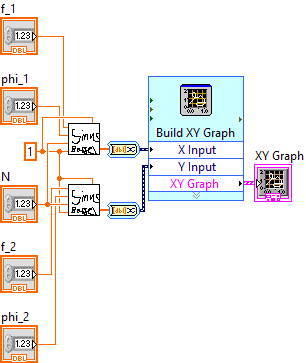
\includegraphics[width=1.0\textwidth]{EIRE2018Dateien/Tag1/lissajous-bilder/Lissajousd}
		\caption{Dargestellt ist das Blockdiagramm und der LabVIEW-Programmcode, mit dem sich Lissajous-Figuren realisieren lassen.}
		\label{lissajousprogrammcode}
	\end{figure}

	\noindent Für die Amplituden soll einfachheitshalber $A_1 = A_2 = 1$ gelten.

	\begin{figure}[H]
		\centering
		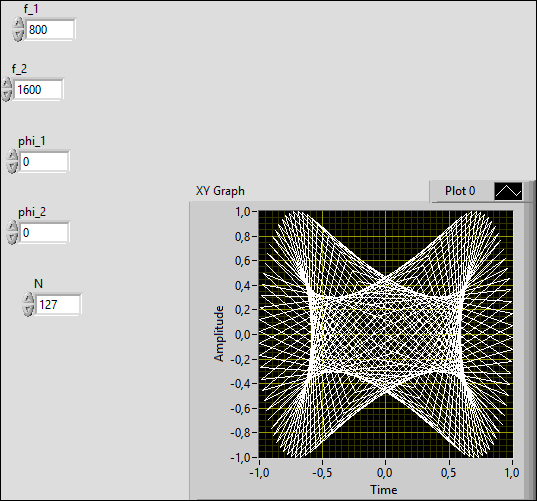
\includegraphics[width=1.0\textwidth]{EIRE2018Dateien/Tag1/lissajous-bilder/Lissajousp}
		\caption{Die Abbildung zeigt das Frontpanel, in dem sich im Anzeigeelement eine Lissajous-Figur befindet. Auf der linken Seite können die entsprechenden $f_1$-, $f_2$-, $\varphi_1$-, $\varphi_2$- und $N$-Werte abgelesen werden.}
		\label{lissajous}
	\end{figure}
	
	\section{Tag 2}
	
	\subsection{Digitales Oszilloskop mit ExpressVI}
	Es wird ein Funktionsgenerator verwendet.
	Dessen Signal wird über einen Analog-Digital-Wandler durch den Computer erfasst.
	Zunächst wird das Signal in LabView mit dem entsprechenden ExpressVI verarbeitet.
	Das zugehörige Programm ist in \cref{fig_tag2_oszi_express_block} und die Frontplatte in \cref{fig_tag2_oszi_express_front} dargestellt.
	
	\begin{figure}[H]  
		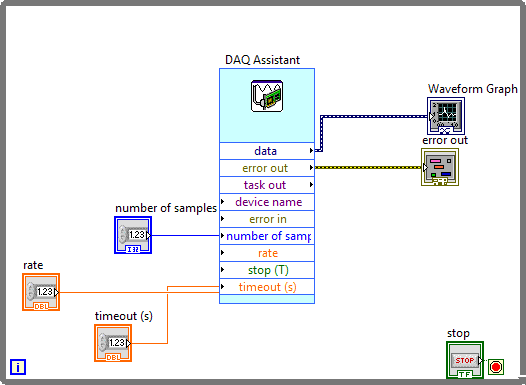
\includegraphics[width=1\textwidth]{EIRE2018Dateien/Tag2/expressVI_1d}
		\centering
		\caption{
			Einfaches Oszilloskop mithilfe des ExpressVIs zur Verarbeitung von Daten von Messgeräten.
		}
		\label{fig_tag2_oszi_express_block}
		\centering
	\end{figure}
	\begin{figure}[H]  
		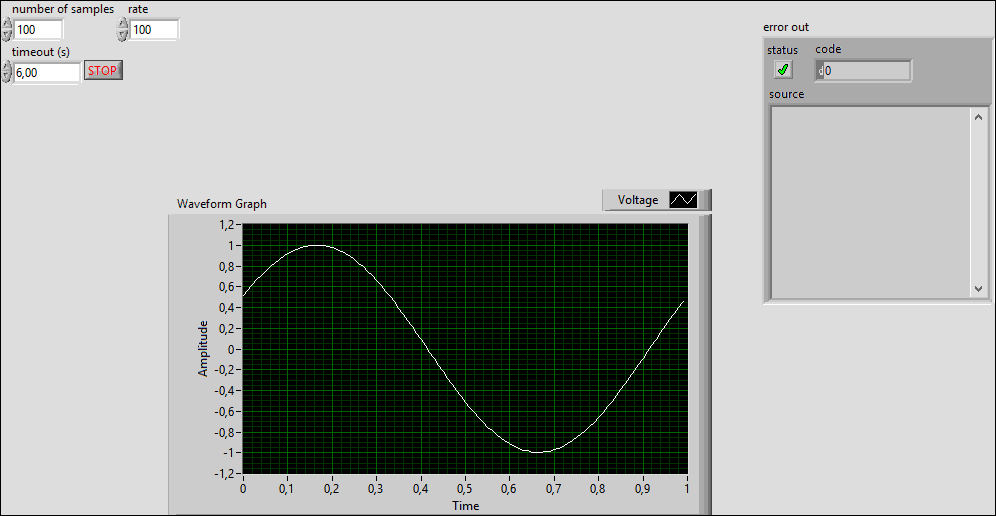
\includegraphics[width=1\textwidth]{EIRE2018Dateien/Tag2/expressVI_1p}
		\centering
		\caption{
			Frontplatte des einfachen Oszilloskop mithilfe des ExpressVIs zur Verarbeitung von Daten von Messgeräten. Dabei wurde durch den Funktionsgenerator ein sinusförmiges Signal ausgegeben.
		}
		\label{fig_tag2_oszi_express_front}
	\centering
	\end{figure}
	
	\subsection{Fouriertheorem} %kp, ob man so Theorie wiedergeben soll und ob man das mit Bindestrich schreibt.
	Gemäß des Fouriertheorems kann jede periodische Funktion als Fourierreihe bzw. Fourierintegral ausgedrückt werden.
	Dies ist nützlich bei der Zerlegung eines möglicherweise verrauschten Signals in seine Bestandteile.
	Das grundsätzliche Problem hierbei ist, dass Messprozesse immer zeitlich begrenzt ist, weshalb das Signal nicht bis in die positive und negative Unendlichkeit periodisch sein kann.
	Dies verursacht den sogenannten \enquote{Leakage-Effekt}, auf den in \cref{leakage} näher eingegangen wird.
	
	\subsection{Abtasttheorem}
	%TODO kurze Zusammenfassung seiner Theorie-Sachen, hab ich auf Papier
	Um ein Signal abzutasten, werden im Analog-Digital-Wandler mithilfe einer Sample-and-Hold-Schaltung zeitlich diskrete Messungen durchgeführt.
	Dies lässt sich als Multiplikation des Signals mit einem Delta-Kamm ausdrücken.
	Dabei treten Summen- und Differenzfrequenzen der Abtastfrequenz (und deren Oberfrequenzen) und den Frequenzen im Signal auf.
	Im Frequenzraum ergibt sich hierdurch eine periodische Fortsetzung des Spektrums des ursprünglichen Signals, wobei die Periode der Abtastfrequenz entspricht, wobei auch die Differenzfrequenzen auftauchen. %TODO ist bissl unschön und man braucht vmtl. ein Bild. Ich weiß aber auch nicht, in wiefern man die Theorie noch mal aufrollen soll.
	Wenn die Abtastfrequenz hinreichend groß ist, kann man nun mithilfe eines Tiefpasses das Signal herausfiltern.
	Dazu muss sie allerdings größer als das Doppelte der höchsten im Signal auftretenden Frequenz sein, da sich ansonsten das Spektrum des Signals mit den Differenzfrequenzen der nächsten Periode überlagern.
	Dies bezeichnet man als Aliasing.
	
	
	\section{Tag 3}
	%eig. zunächst Fertigstellung von Tag2 Teil 1
	\subsection{Leakage-Effekt und Fensterfunktion}
	\label{leakage}
	Wenn die Signalfrequenz kein Vielfaches des Produkts aus Abtastfrequenz und Zahl an Messpunkten pro Messung ist, tritt aufgrund der Endlichkeit des Messprozesses der sogenannte \enquote{Leakage-Effekt} auf. %TODO Bild?
	%https://de.wikipedia.org/wiki/Datei:Spectral_leakage_Sine.svg
	Dieser verursacht eine Verbreiterung des Peaks der Signalfrequenz im Frequenzbild.
	Um diesen Effekt zu minimieren können Fensterfunktionen angewendet werden.
	Im Folgenden wird das \enquote{Von-Hann-Fenster} (auch \enquote{Hanning-Fenster}) verwendet. %mehr erklären? Hat er halt auch nicht so schöne gemacht, nur halt 1-cos
	
	\subsection{Digitales Oszilloskop ohne ExpressVI} % hier ist halt die Tagreihenfolge bissl gebrochen. Ich glaube, wir haben das an Tag 2 angefangen und Tag 3 beendet
	Das Oszilloskopprogramm von zuvor wird ersetzt durch eines, dass anstelle des ExpressVIs Konfiguration, Messung und Cleanup getrennt enthält.
	Dieses ist in \cref{fig_tag23_oszi_manuell_block} dargestellt, während in \cref{fig_tag23_oszi_manuell_front} die Frontplatte bei einem Eingangssignal von \SI{600}{\hertz}.
	
	\begin{figure}[H]  
		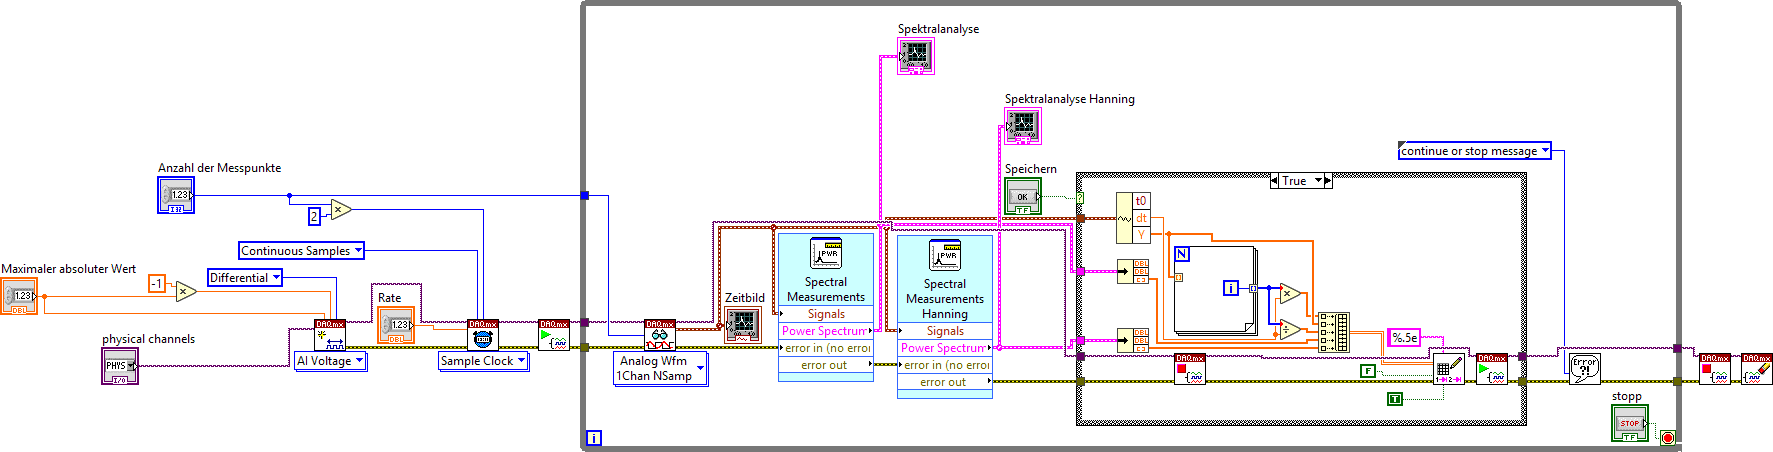
\includegraphics[width=1\textwidth]{EIRE2018Dateien/Tag3/ManuellVId}
		\centering
		\caption{
			Oszilloskopprogramm, das eine Abtastung vornimmt und das Ergebnis im Zeitbild sowie im Frequenzbild mit und ohne Hann-Fenster darstellt.
			Außerdem ist die Speicherung der Daten in einem Textdokument ermöglicht.
		}
		\label{fig_tag23_oszi_manuell_block}
		\centering
	\end{figure}

	\begin{figure}[H]  
		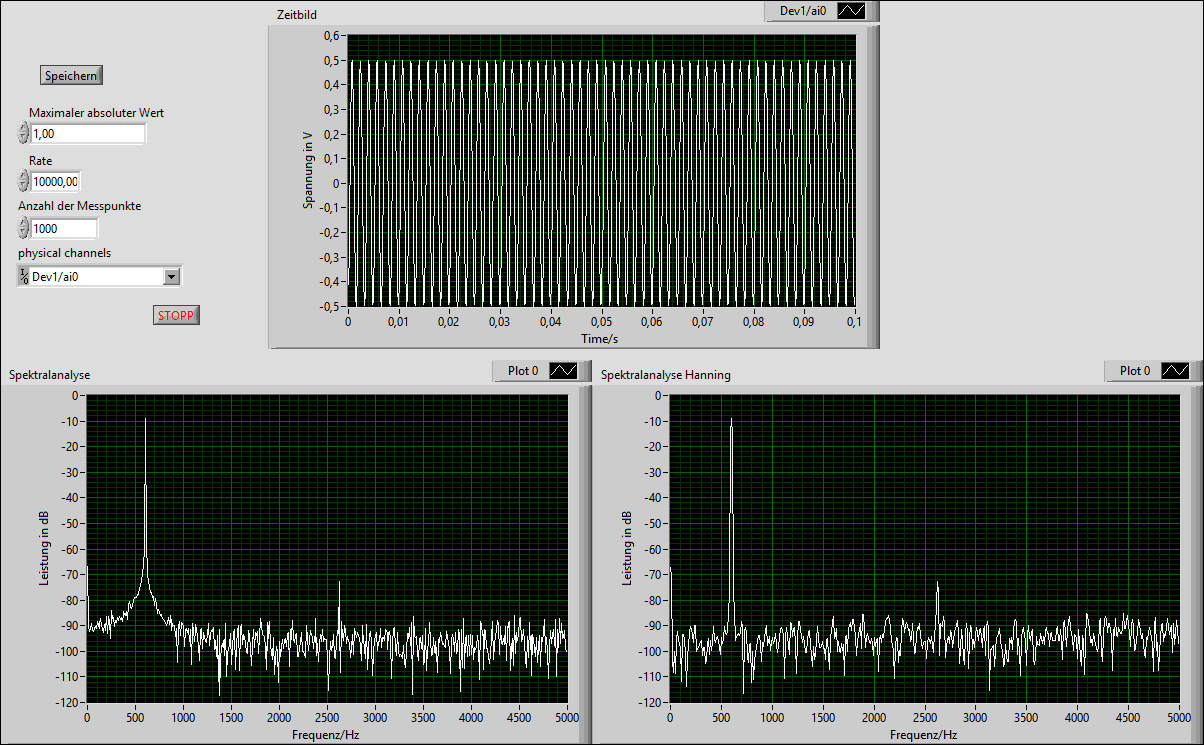
\includegraphics[width=1\textwidth]{EIRE2018Dateien/Tag3/ManuellVIp}
		\centering
		\caption{
			Oszilloskopfrontplatte. Dargestellt wird das gemessene Signal im Zeitbild sowie im Frequenzbild mit und ohne Von-Hann-Fenster. Einstellbar ist die Abtastfrequenz, die Anzahl der Messpunkte, der Eingangskanal des Messgerätes und der maximale messbare Wert, wobei der minimale auf das Negative des maximalen gesetzt wird.
			Mithilfe des Stopp-Knopfes kann das Programm gestoppt werden und mit dem Speichern-Knopf werden die aktuellen Messwerte aus allen drei Diagrammen in eine Textdatei exportiert.
		}
		\label{fig_tag23_oszi_manuell_front}
		\centering
	\end{figure}

	Hierbei wurde ebenfalls die Möglichkeit die aktuellen Messwerte zu speichern eingeführt.
	Dazu wurden die Strukturen, die in den Diagrammen dargestellt werden in ihre Bestandteile zerlegt und die Arrays der Y-Werte mit zwei Arrays für fortlaufende Zeit- und Frequenzwerte kombiniert und der Speicherfunktion zugeführt.
	Der Speichervorgang befindet sich innerhalb eines case-Konstrukts, das ignoriert wird, solange der Speichern-Knopf nicht gedrückt wurde.
	Außerdem werden Fehlermeldungen einer Fehlerdialogfunktion zugeführt, die dem Nutzer erlaubt bei Fehlern wahlweise das Programm anzuhalten oder weiterlaufen zu lassen.
	Um ein Volllaufen des Mess-Buffers zu vermeiden, wird dieser doppelt so groß wie die Anzahl der Messpunkte pro Zyklus gewählt.
	
	\subsection{Aliasing}
	Um den Effekt des Aliasings absichtlich herbeizuführen, werden bei einer Abtastfrequenz von \SI{1000}{\hertz} zwei verschiedene Signale abgetastet.
	Da bei dieser Abtastfrequenz die höchste Frequenz im Signal kleiner als \SI{500}{\hertz} sein muss, ist hierbei zu erwarten, dass ein Signal von \SI{400}{\hertz} korrekt abgetastet wird, während eines mit \SI{600}{\hertz} falsch abgetastet wird.
	Das Spektrum des abgetasteten Signals bei diesen beiden Signalfrequenzen ist in \cref{fig_ali} dargestellt.
	
	\begin{figure}[H]
		\centering
		\begin{subfigure}[t]{0.5\textwidth}
			\centering
			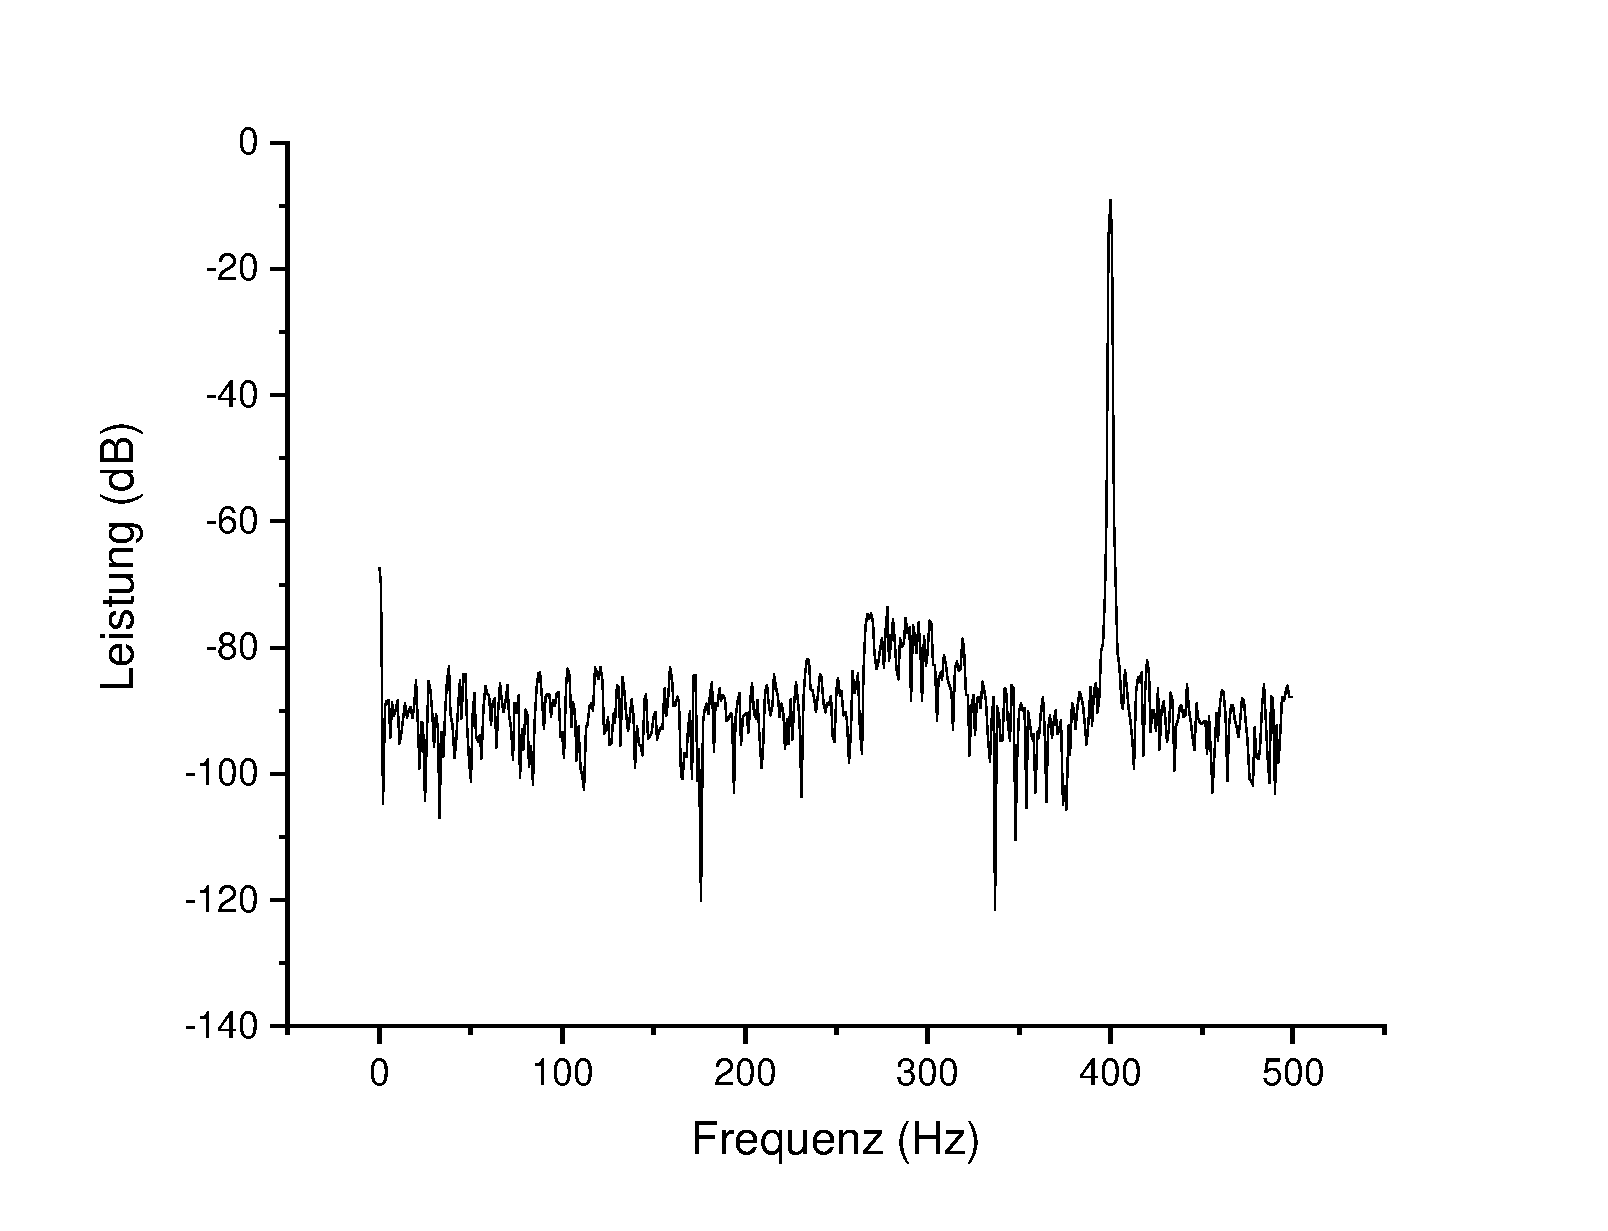
\includegraphics[width=1\textwidth]{Origin-Files/aliasing_abtast1000bei400sig}
			\caption{\SI{400}{\hertz}}
		\end{subfigure}%
		\begin{subfigure}[t]{0.5\textwidth}
			\centering
			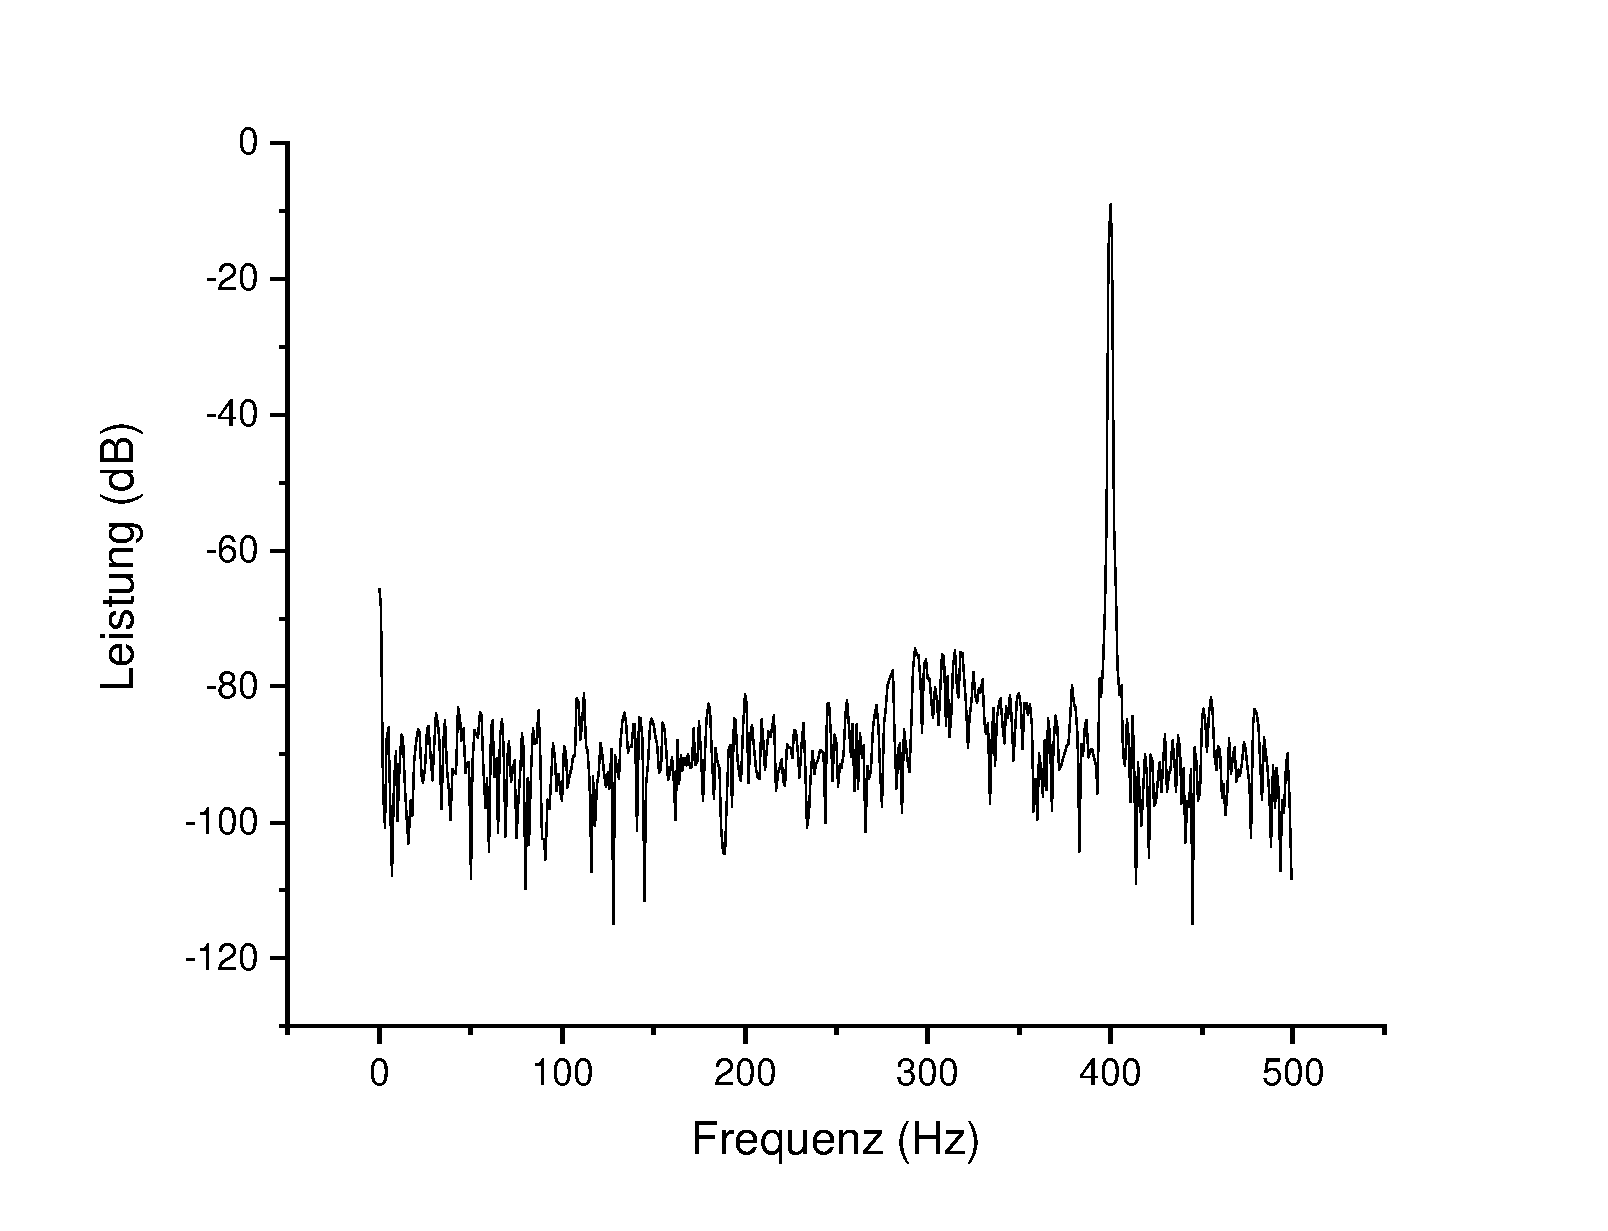
\includegraphics[width=1\textwidth]{Origin-Files/aliasing_abtast1000bei600sig}
			\caption{\SI{600}{\hertz}}
		\end{subfigure}
		\label{fig_ali}
		\caption{Mit einer Abtastfrequenz von \SI{1000}{\hertz} abgetastete Signale, deren Frequenz einmal \SI{400}{\hertz} und einmal \SI{600}{\hertz} beträgt, sodass einmal korrekt und einmal falsch abgetastet wird.}
		\centering
	\end{figure}
	
	Es fällt auf, dass sich zwischen diesen beiden Signalen kein Unterschied erkennen lässt.
	Dies liegt daran, dass bei einer Signalfrequenz von \SI{600}{\hertz} die eigentliche Signalfrequenz nicht mehr vom idealen Tiefpass übertragen wird, während die Differenzfrequenz von Abtastfrequenz und Signalfrequenz \SI{400}{\hertz} beträgt.
	Es ist an den beiden Signalen zu erkennen, dass sich ein falsch abgetastetes Signal nicht mehr von einem korrekt abgetasteten Signal bei der entsprechenden Differenzfrequenz unterscheiden lässt.
	Man stellt fest, dass man vor der Abtastung bereits wissen muss, welche Frequenzen im Signal vorkommen. 
	
	
	\subsection{Amplitudenmodulierte Signale} %SoundkarteOuszi
	
	\subsubsection{Erzeugung} %TODO hier ansetzen mit EIRE2018Dateien/Tag3/Soundkarteoutoszi
	% + Ausgabe über Soundkarte
	
	Es soll nun ein amplitudenmoduliertes Signal erzeugt werden und über die Soundkarte des verwendeten PCs ausgegeben werden.
	Dabei wird das Signal der Soundkarte wieder auf den Analog-Digital-Wandler gegeben und mit dem zuvor erstellten Oszilloskopprogramm verarbeitet.
	In \cref{fig_tag3_am_soundkarte_block} ist das dazu verwendete LabView-Programm dargestellt.
	Moduliert werden soll die Überlagerung zweier Signale mit einstellbarer Frequenz und Amplitude.
	Auch Trägerfrequenz und Modulationsgrad soll einstellbar sein.
	Die Amplitudenmodulation lässt sich durch die Gleichung
	\begin{equation}
		S_{AM}(t)=S_T (1+m \cdot s_s(t)) \cdot \cos(2\pi f_T t)
	\end{equation}
	beschreiben.
	Da die Überlagerung von zwei sinusförmigen Signalen beliebiger aber fester Frequenz moduliert werden soll gilt:
	\begin{equation}
		s_s(t) = A_1 \cos (2\pi f_1 t) + A_2 \cos (2\pi f_2 t)
	\end{equation}
	
	Diese beiden Gleichungen sollen im Folgenden durch Operationen auf Arrays realisiert und als Audiosignal ausgegeben werden.	
	Dazu wird das in \cref{sinusfkt} erstellte Programm verwendet, um Arrays von Sinusfunktionen zu erstellen.
	Diesem wird in jedem Fall die Phase 0 zugeführt und 44100 Stützstellen gewählt, weil dies der Abtastrate bei CDs entspricht.%TODO fact-Check,ob das wirklich cd audio abtast ist und Logik-Check, ob man das wirklich deswegen macht.
	Dem Programm wird zunächst eine Amplitude von 1 gegeben und dann werden alle Array-Elemente mit der gewählten Phase multipliziert.
	Dies hängt lediglich damit zusammen, dass zuvor im Sinus-erstellenden Programm ein Fehler  vorhanden war, der dies nötig machte. %TODO Jannik, sachma, ob das ok ist. Ich finds unschöne, weil plötzlich imperfekt, aber ich hab keine bessere Lösung und müsste man maybe oben bei den Sinusbessel anmerken, dass da der Fehler war und der später gefixt wurde
	In \cref{fig_tag3_am_soundkarte_block} ist zu erkennen, dass zunächst zwei Sinus-Arrays erstellt werden, für die jeweils eine Signalfrequenz und -amplitude gewählt werden.
	Die beiden resultierenden Arrays werden addiert, mit dem Modulationsgrad multipliziert und dann mit dem Array der Trägerfrequenz multipliziert.
	Dieses wurde zuvor in gleicher Art und Weise mit der Trägerfrequenz erstellt.
	Für die Amplitude des Trägersignals wird der Kehrwert der maximalen Signalamplitude gewählt, damit die resultierende Amplitude immer auf 1 liegt, da die Soundkarte höhere Werte nicht verarbeitet.
	Das resultierende Array wird im Zeit- und Frequenzbild dargestellt und dann mithilfe der entsprechenden VIs über die Soundkarte ausgegeben. %TODO sicherstellen, dass vorher irgendwo steht dass VI für visual instrument oder so steht.
	
	
	\begin{figure}[H]  
		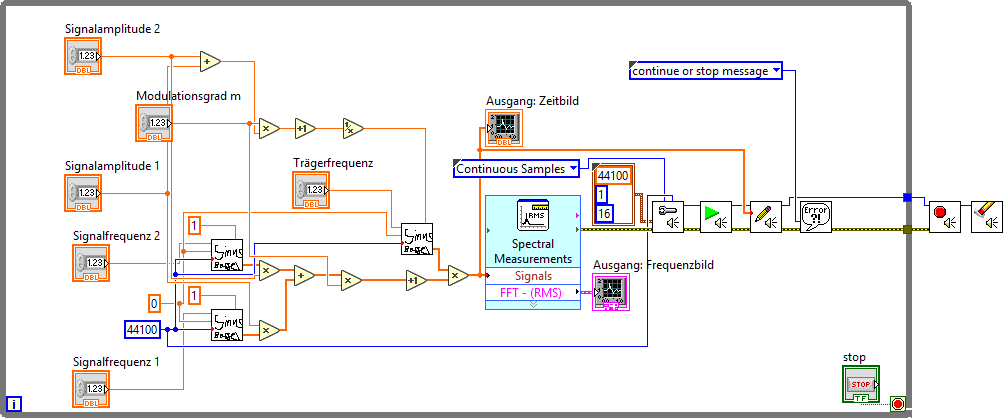
\includegraphics[width=1\textwidth]{EIRE2018Dateien/Tag3/Soundkarteoutoszi/AMd}
		\centering
		\caption{
			Blockdiagramm des Programms zur Erzeugung eines amplitudenmodulierten Signals und Ausgabe dessen über die Soundkarte.
		}
		\label{fig_tag3_am_soundkarte_block}
		\centering
	\end{figure}
	
	\begin{figure}[H]  
		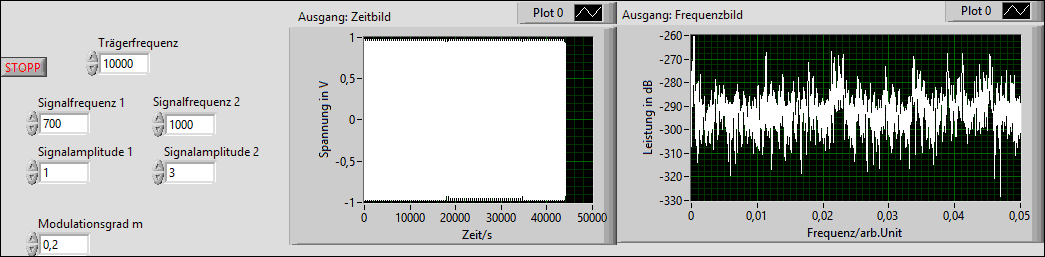
\includegraphics[width=1\textwidth]{EIRE2018Dateien/Tag3/Soundkarteoutoszi/AMp}
		\centering
		\caption{
			Frontplatte des Programms zur Erzeugung eines amplitudenmodulierten Signals und Ausgabe dessen über die Soundkarte.
		}
		\label{fig_tag3_am_soundkarte_front}
		\centering
	\end{figure}

	\begin{figure}[H]  
		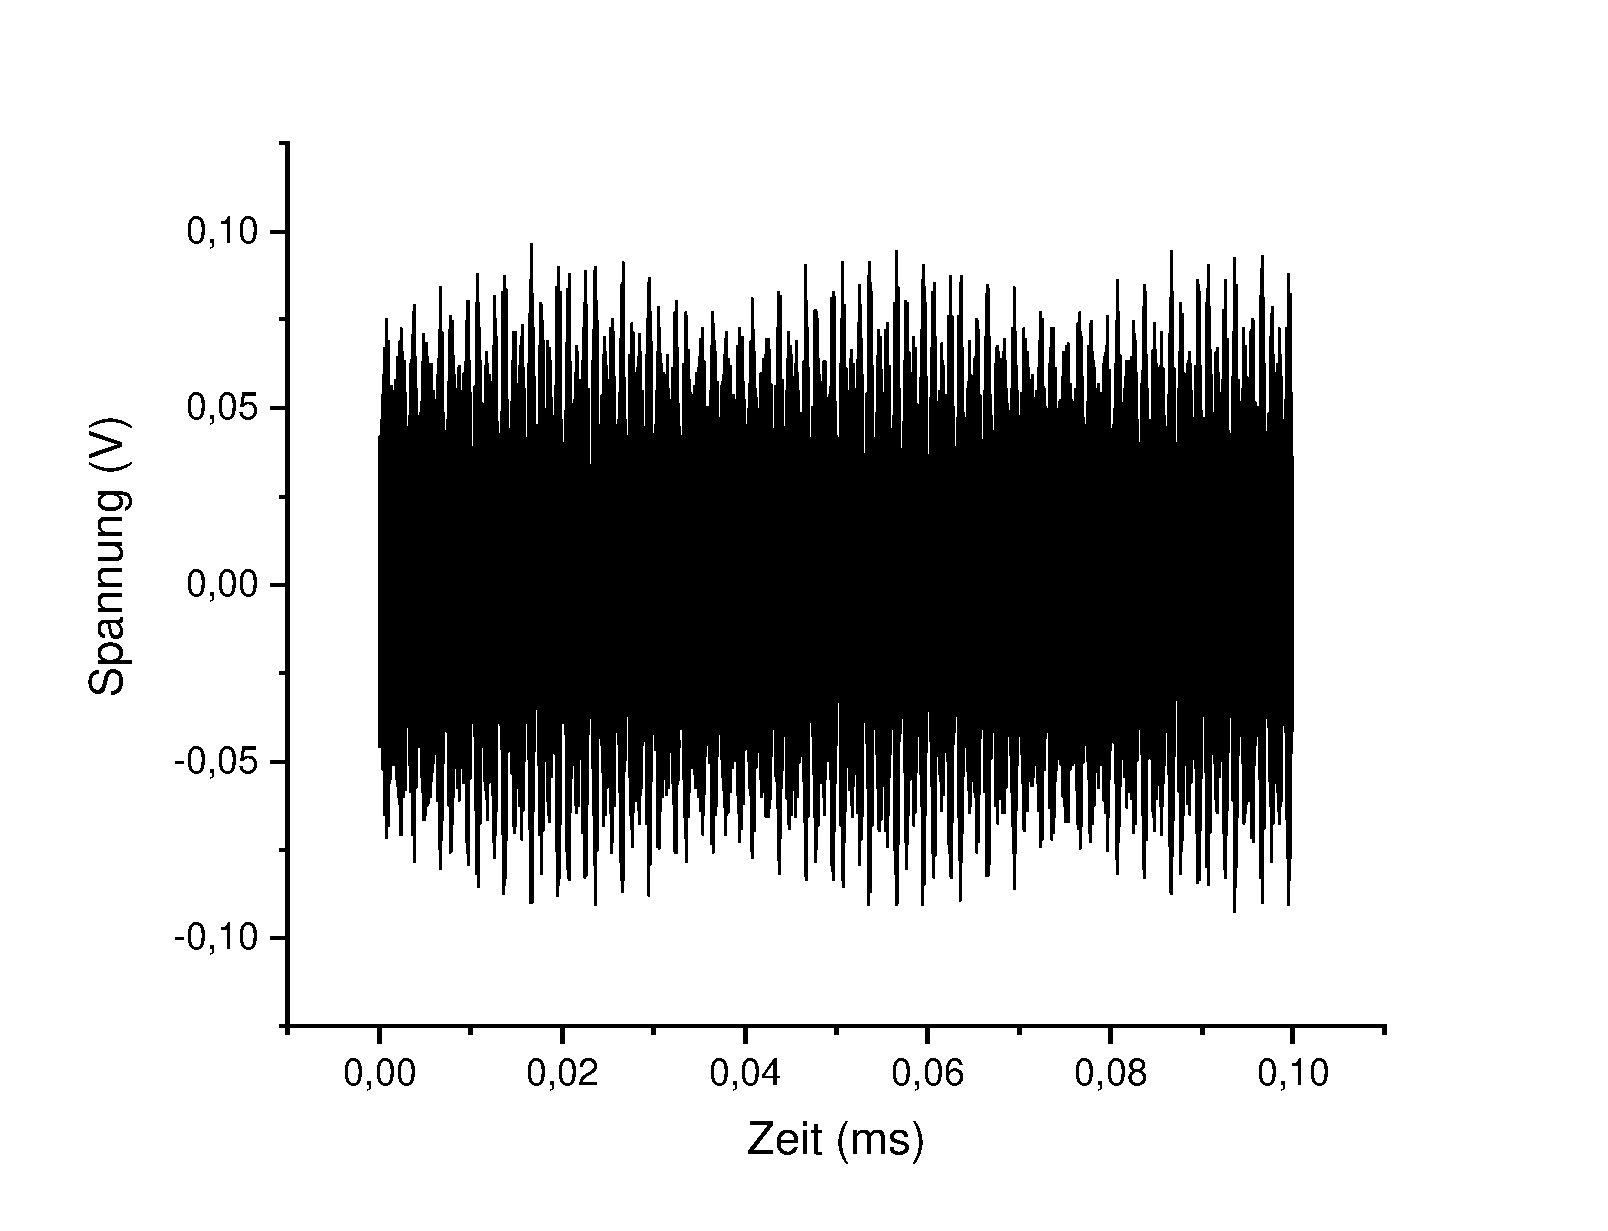
\includegraphics[width=0.7\textwidth]{Origin-Files/AM-Zeit}
		\centering
		\caption{
			Ausgabe des Oszilloskopprogramms im Zeitraum bei Erfassung des amplitudenmodulierten Signals, das mittels der Soundkarte ausgegeben wird.
		}
		\label{fig_tag3_am_soundkarte_zeit}
		\centering
	\end{figure}
	
	\begin{figure}[H]  
		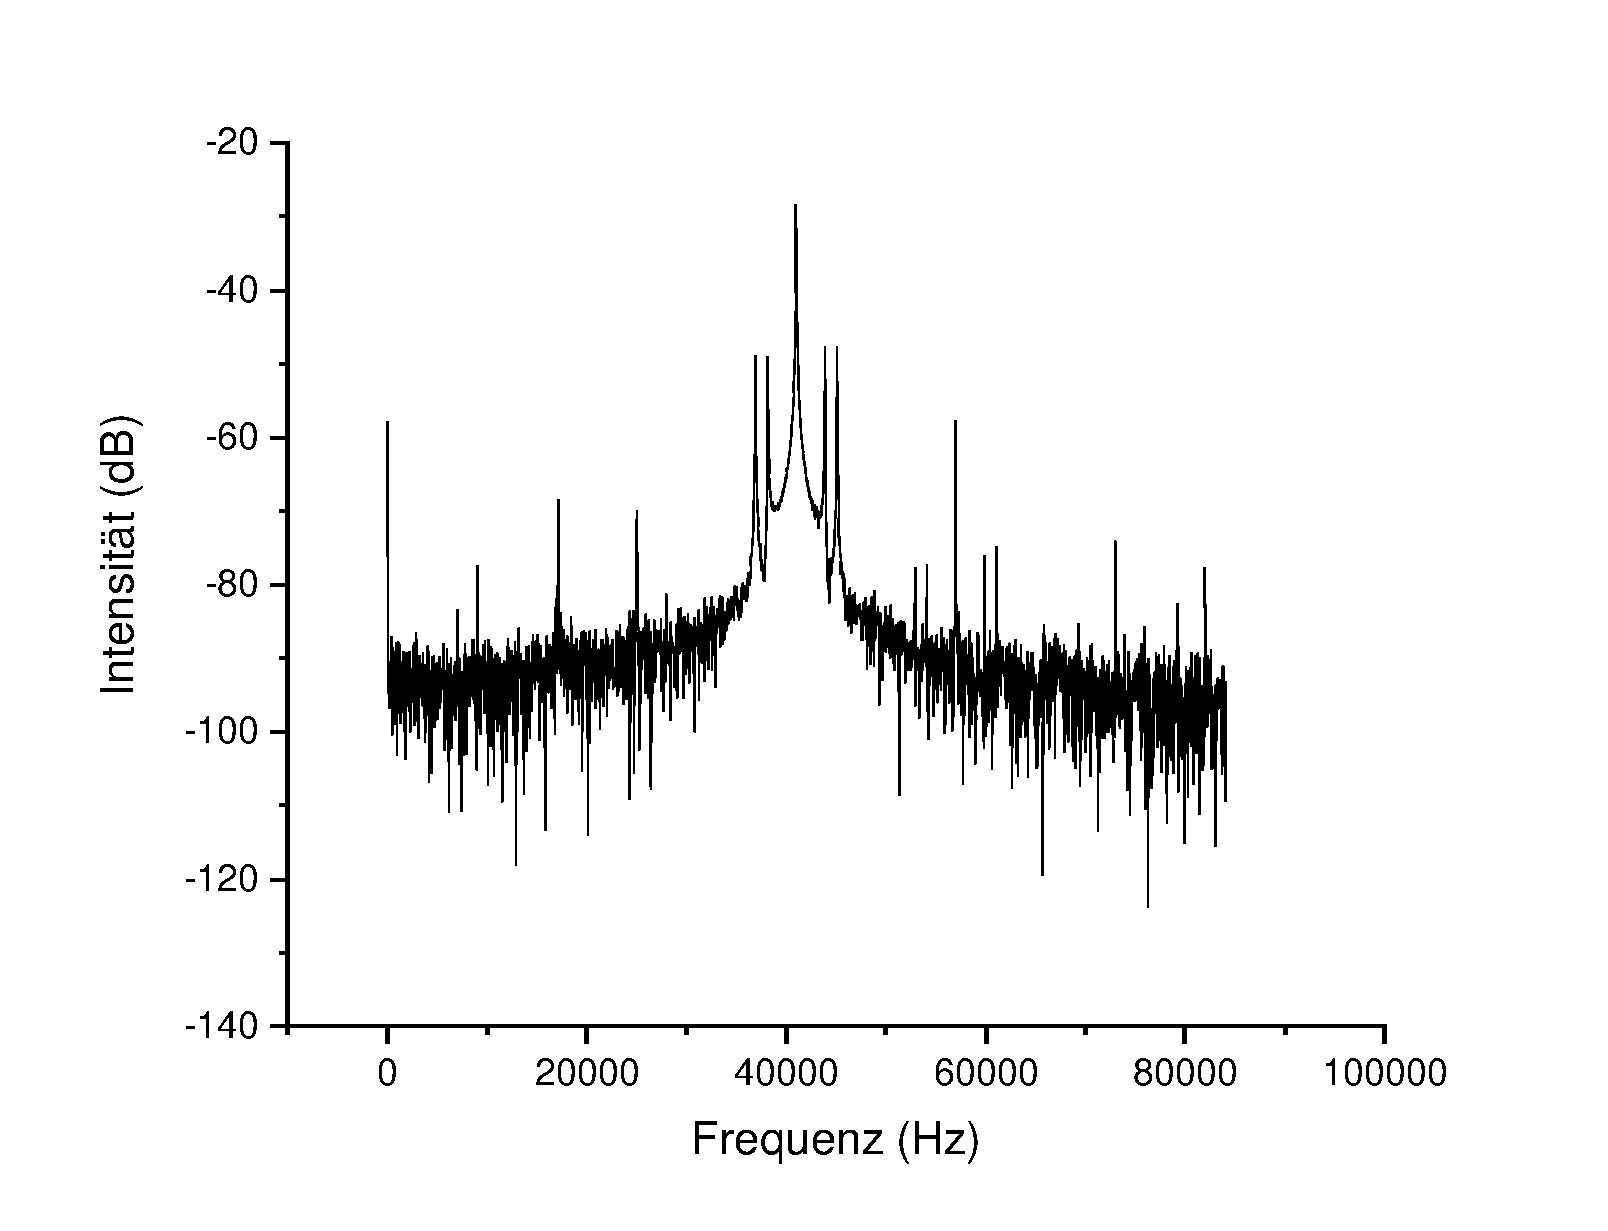
\includegraphics[width=0.7\textwidth]{Origin-Files/AM-Freq-Hann}
		\centering
		\caption{
			Ausgabe des Oszilloskopprogramms im Frequenzraum bei Erfassung des amplitudenmodulierten Signals, das mittels der Soundkarte ausgegeben wird.
		}
		\label{fig_tag3_am_soundkarte_freq}
		\centering
	\end{figure}


	\subsubsection{Demodulation}
	%Betrag, Quadrat
	%TODO: unklar wo, aber absichtlicher Leakage und Vielfaches der Abtastfrequenz
	\section{Tag 4}
	
	\subsection{Demodulation eines AM-Signals mittels Trägerfrequenzmultiplikation}
	%zunächst Träger durch Bandpass mit Grenzfrequenzen bei +- 20Hz um geratenen Träger: Vgl. Radio
	%m=0,2 und m=1,2 vergleichen => höherer Modulationsgrad macht höhere Spitzen im Demodulierten
	\begin{figure}[H]
		\centering
		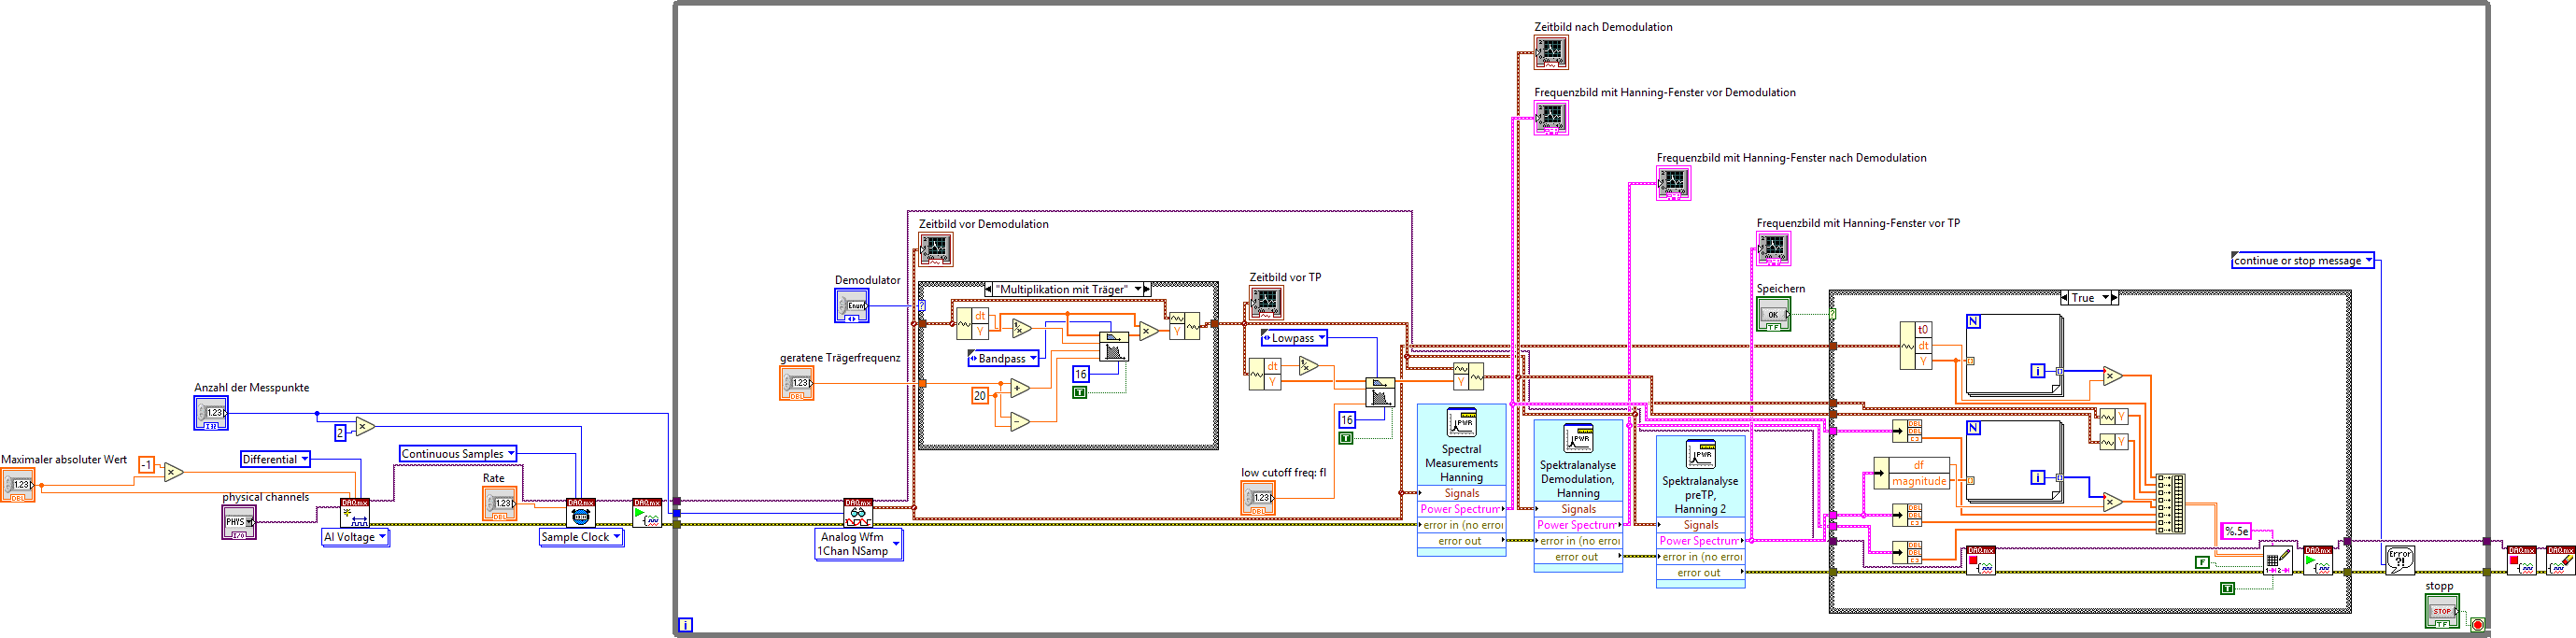
\includegraphics[width=1.0\textwidth]{EIRE2018Dateien/Tag4/traegerMultOszi/Oszilloskop__modifiziertd}
		\caption{.}
	\end{figure}

	\begin{figure}[H]
		\centering
		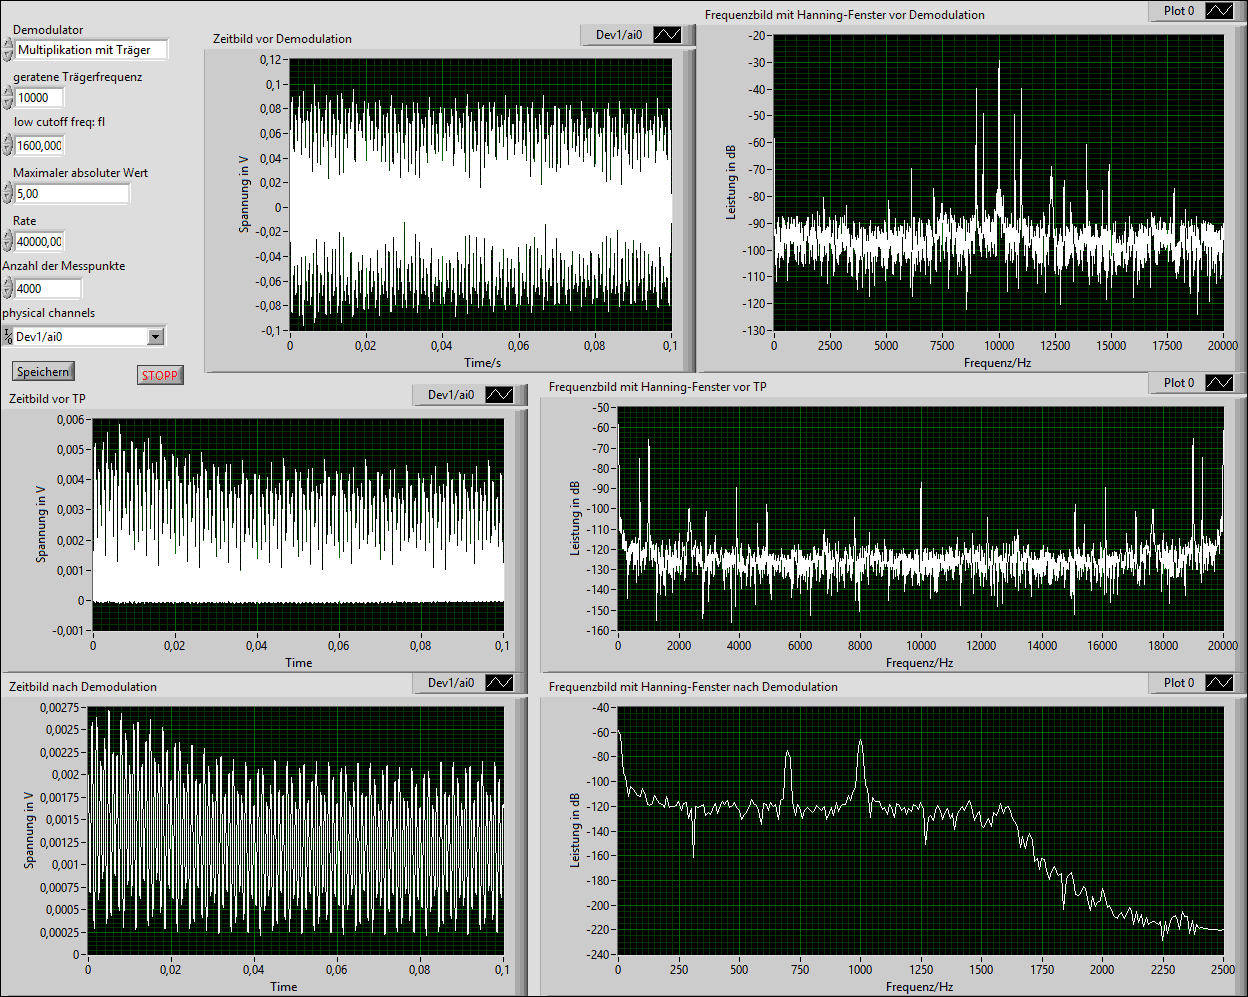
\includegraphics[width=1.0\textwidth]{EIRE2018Dateien/Tag4/traegerMultOszi/Oszilloskop__modifiziertp}
		\caption{.}
	\end{figure}

	\begin{figure}[H]
		\centering
		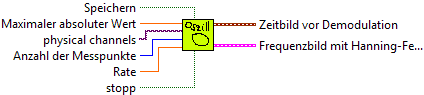
\includegraphics[width=1.0\textwidth]{EIRE2018Dateien/Tag4/traegerMultOszi/Oszilloskop__modifiziertc}
		\caption{.}
	\end{figure}
	
	\subsection{Erzeugung eines phasen- bzw. frequenzmodulierten Signals}
	% Grundlagen AM+FM, Seitenbänder AM, AM größere Bandbreite benötigt
	\begin{figure}[H]
		\centering
		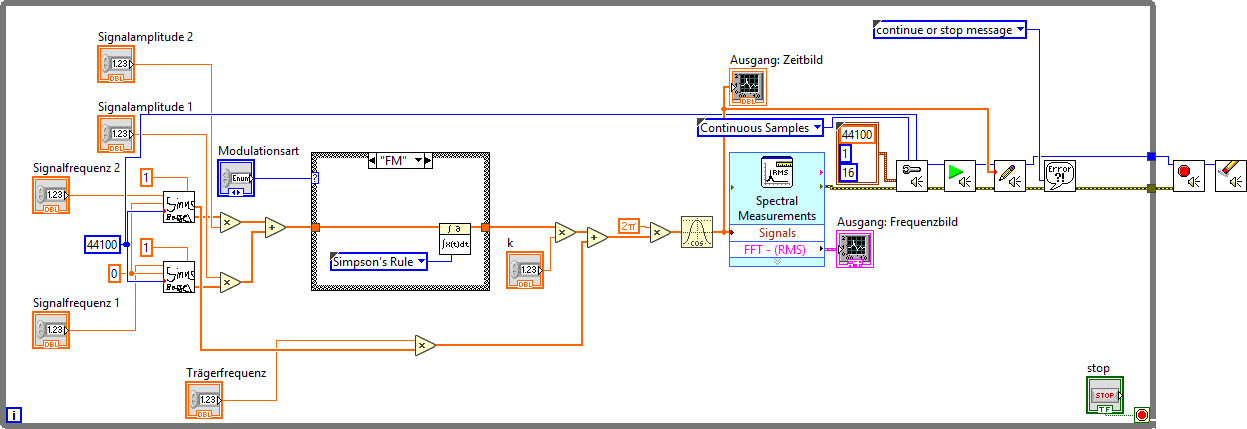
\includegraphics[width=1.0\textwidth]{EIRE2018Dateien/Tag4/FMPM-Erzeugung/FMPM-Erzeugungd}
		\caption{.}
	\end{figure}

	\begin{figure}[H]
		\centering
		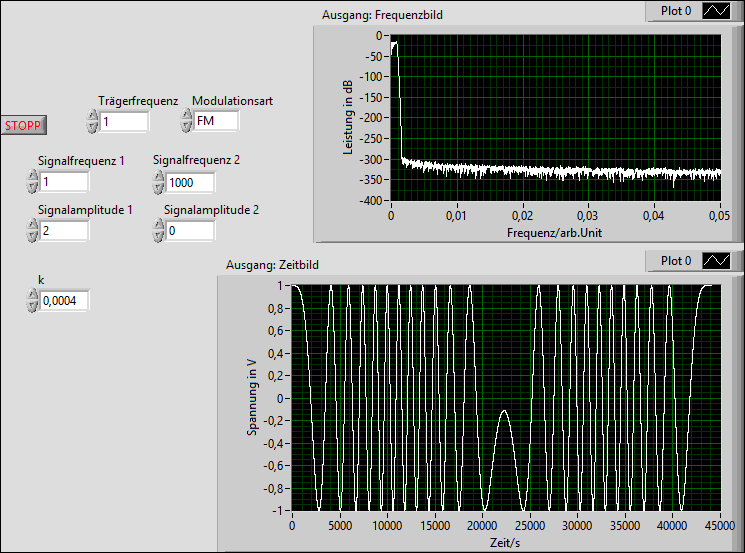
\includegraphics[width=1.0\textwidth]{EIRE2018Dateien/Tag4/FMPM-Erzeugung/FM-FMPM-Erzeugungp}
		\caption{.}
	\end{figure}

	\begin{figure}[H]
		\centering
		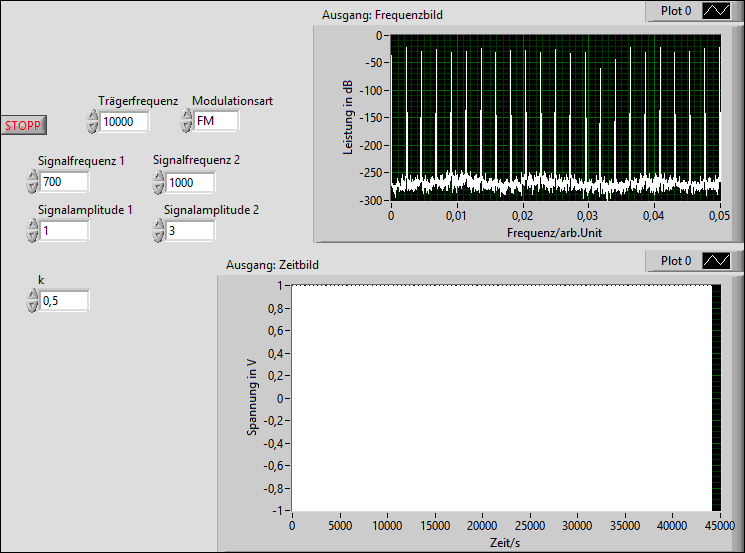
\includegraphics[width=1.0\textwidth]{EIRE2018Dateien/Tag4/FMPM-Erzeugung/anderekbei10000Traegerfr/FM-FMPM-Erzeugungp}
		\caption{.}
	\end{figure}

	\begin{figure}[H]
		\centering
		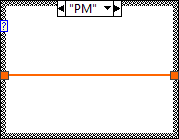
\includegraphics[width=1.0\textwidth]{EIRE2018Dateien/Tag4/FMPM-Erzeugung/PM-FMPM-Erzeugungd1}
		\caption{.}
	\end{figure}

	\begin{figure}[H]
		\centering
		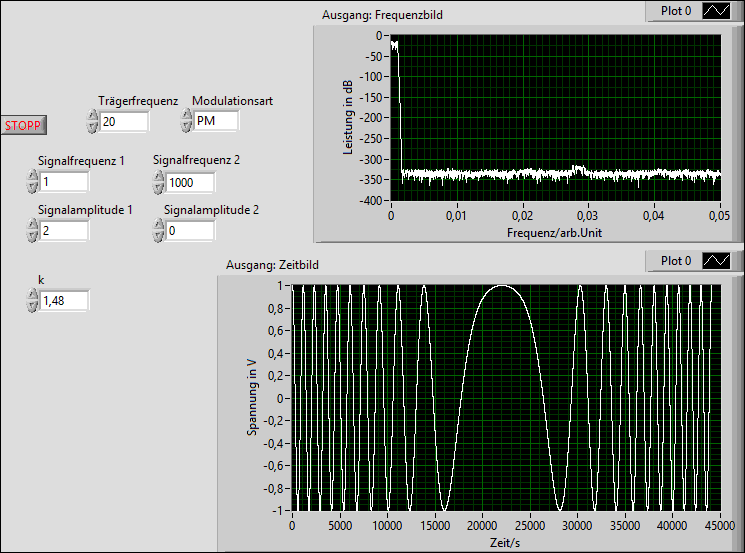
\includegraphics[width=1.0\textwidth]{EIRE2018Dateien/Tag4/FMPM-Erzeugung/PM-FMPM-Erzeugungp}
		\caption{.}
	\end{figure}
	
	\subsection{Demodulation eines phasen- bzw. frequenzmodulierten Signals}
	% 
	\begin{figure}[H]
		\centering
		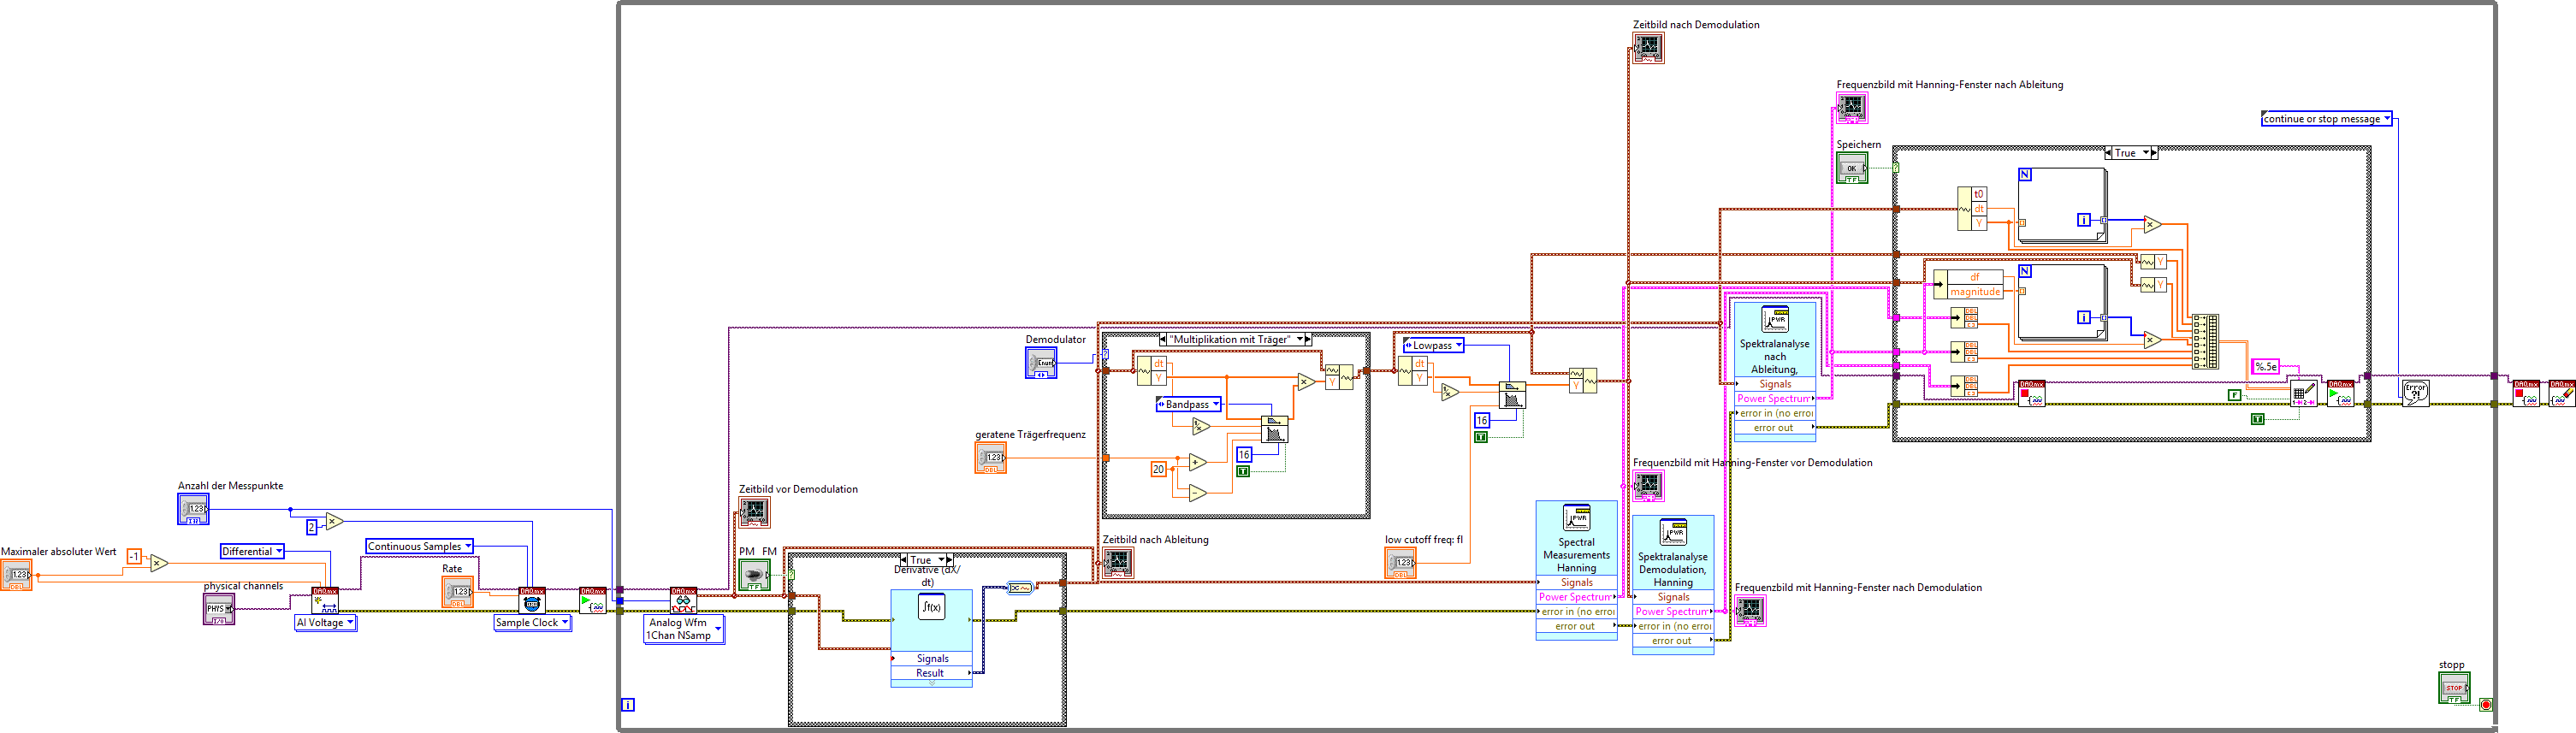
\includegraphics[width=1.0\textwidth]{EIRE2018Dateien/Tag4/OsziFMPM-Demod/FM/OsziPlusFMPMd}
		\caption{.}
	\end{figure}

	\begin{figure}[H]
		\centering
		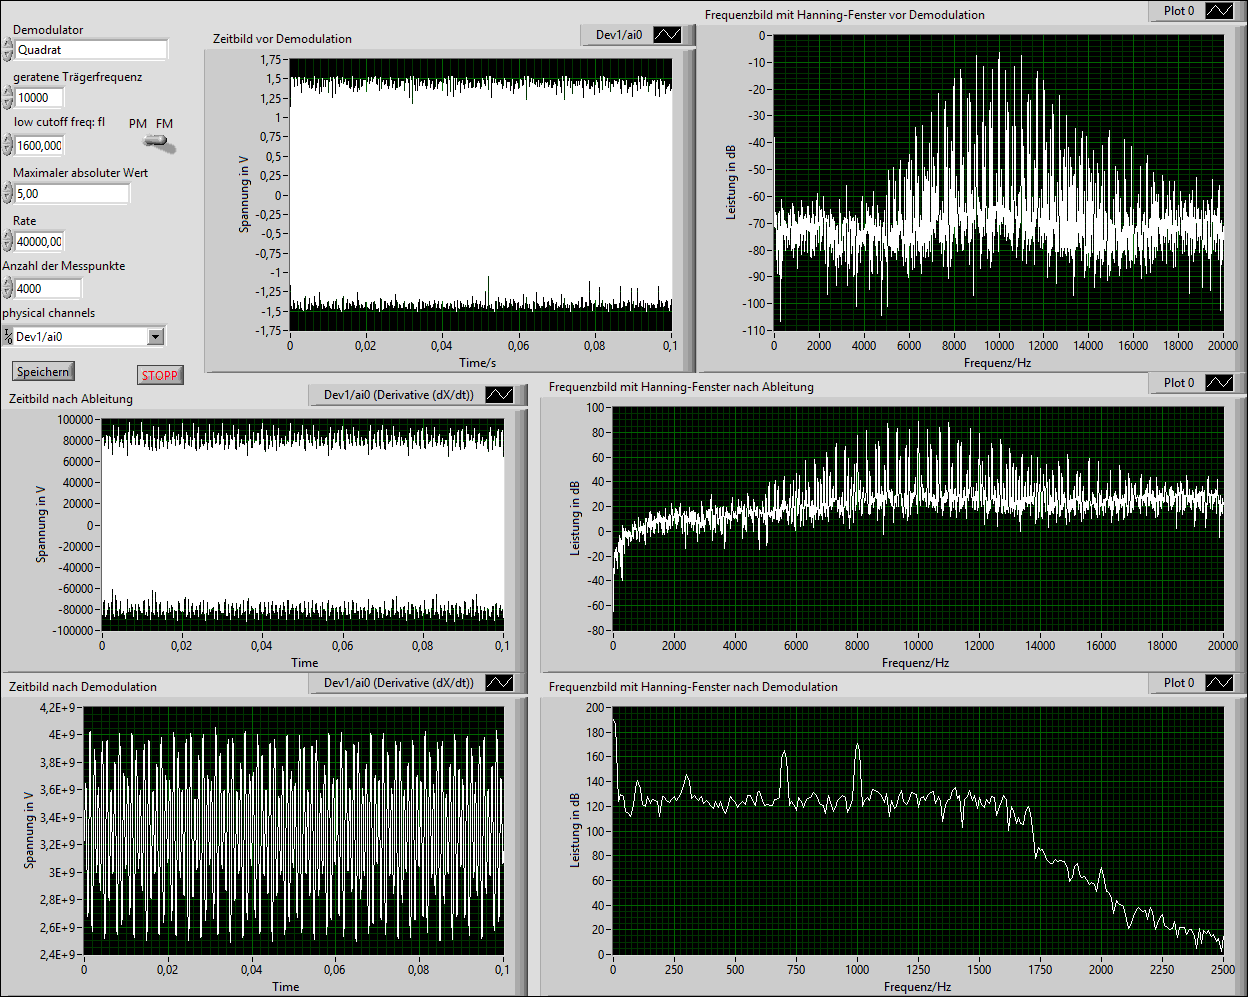
\includegraphics[width=1.0\textwidth]{EIRE2018Dateien/Tag4/OsziFMPM-Demod/FM/OsziPlusFMPMp}
		\caption{.}
	\end{figure}
\iffalse
	\begin{figure}[H] %FM-Diagramm
		\centering
		\includegraphics[width=1.0\textwidth]{}
		\caption{.}
	\end{figure}

	\begin{figure}[H]
		\centering
		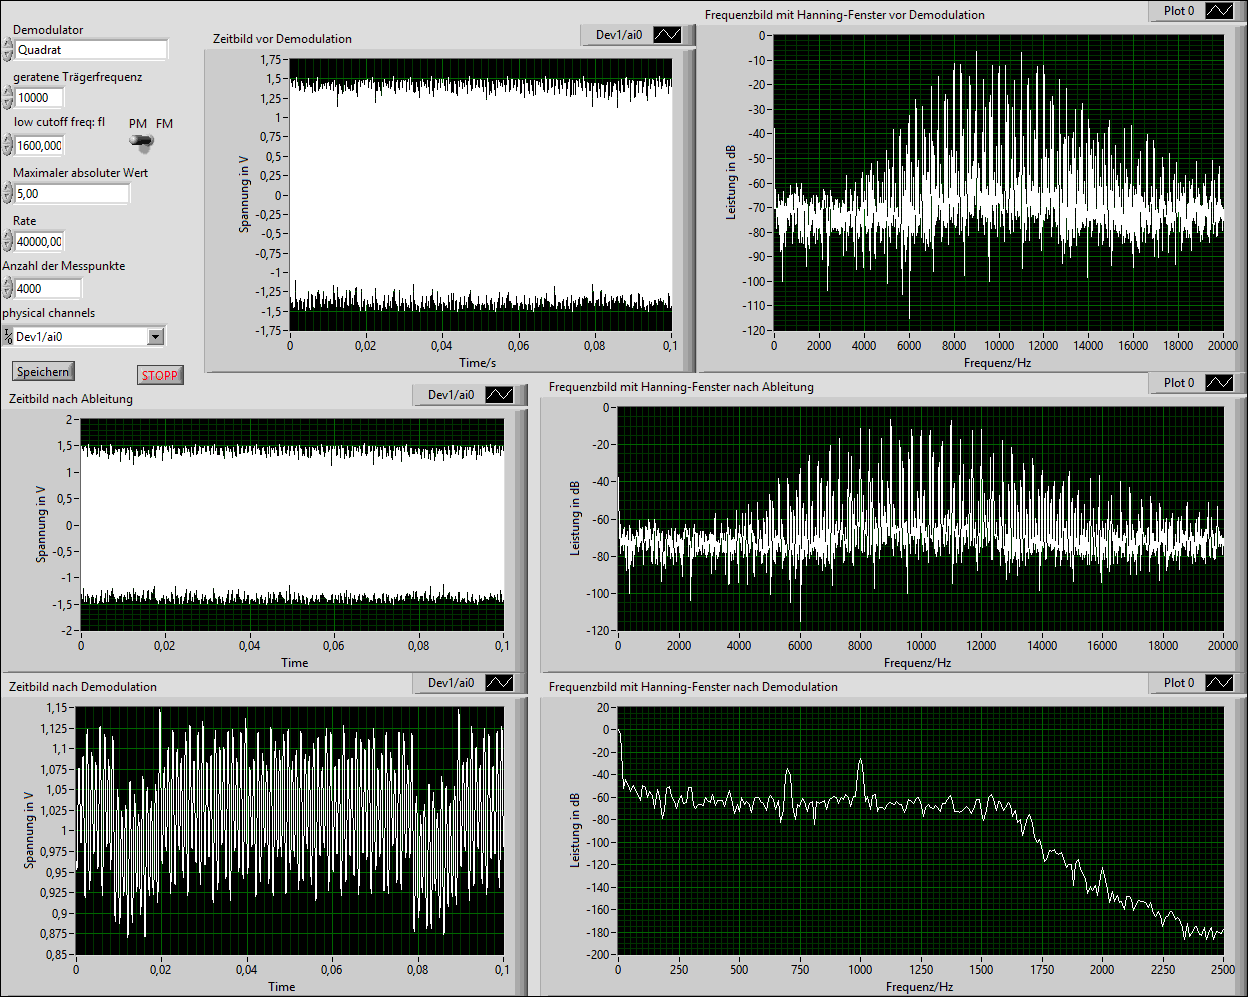
\includegraphics[width=1.0\textwidth]{EIRE2018Dateien/Tag4/OsziFMPM-Demod/PM/OsziPlusFMPMp}
		\caption{.}
	\end{figure}

	\begin{figure}[H] %PM-Diagramm
		\centering
		\includegraphics[width=1.0\textwidth]{}
		\caption{.}
	\end{figure}
\fi
	%Fktion nur schön für bestimmten Bereich von k, weil , wenn zu hoch: zu viele Oberwellen, zu klein: demoduliertes Signal geht im Rauschen unter
	\subsubsection{Erweiterte Demodulation mit Bandpass und zusätzlicher Integration des Signals}
	
	\begin{figure}[H]
		\centering
		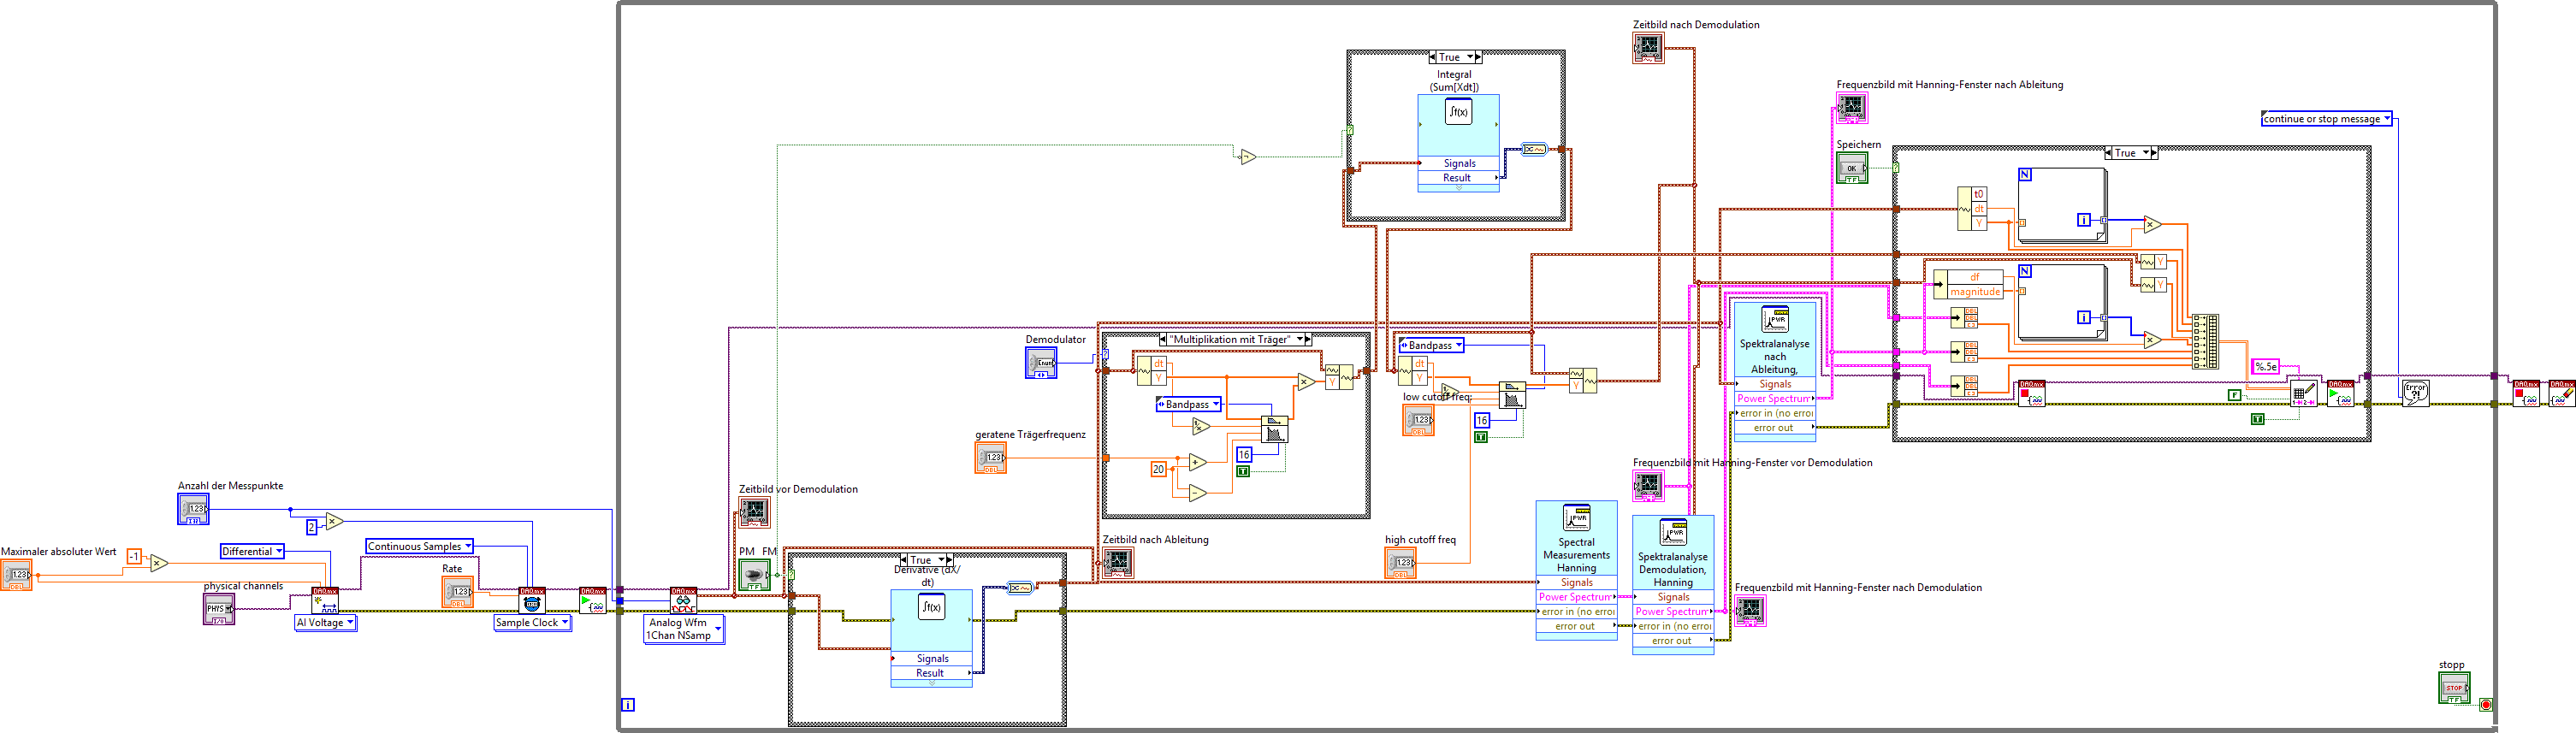
\includegraphics[width=1.0\textwidth]{EIRE2018Dateien/Tag4/OsziFMPM-Demod/mitBandpassUndIntegrationBilder/OsziPlusFMPMd}
		\caption{.}
	\end{figure}

	\begin{figure}[H]
		\centering
		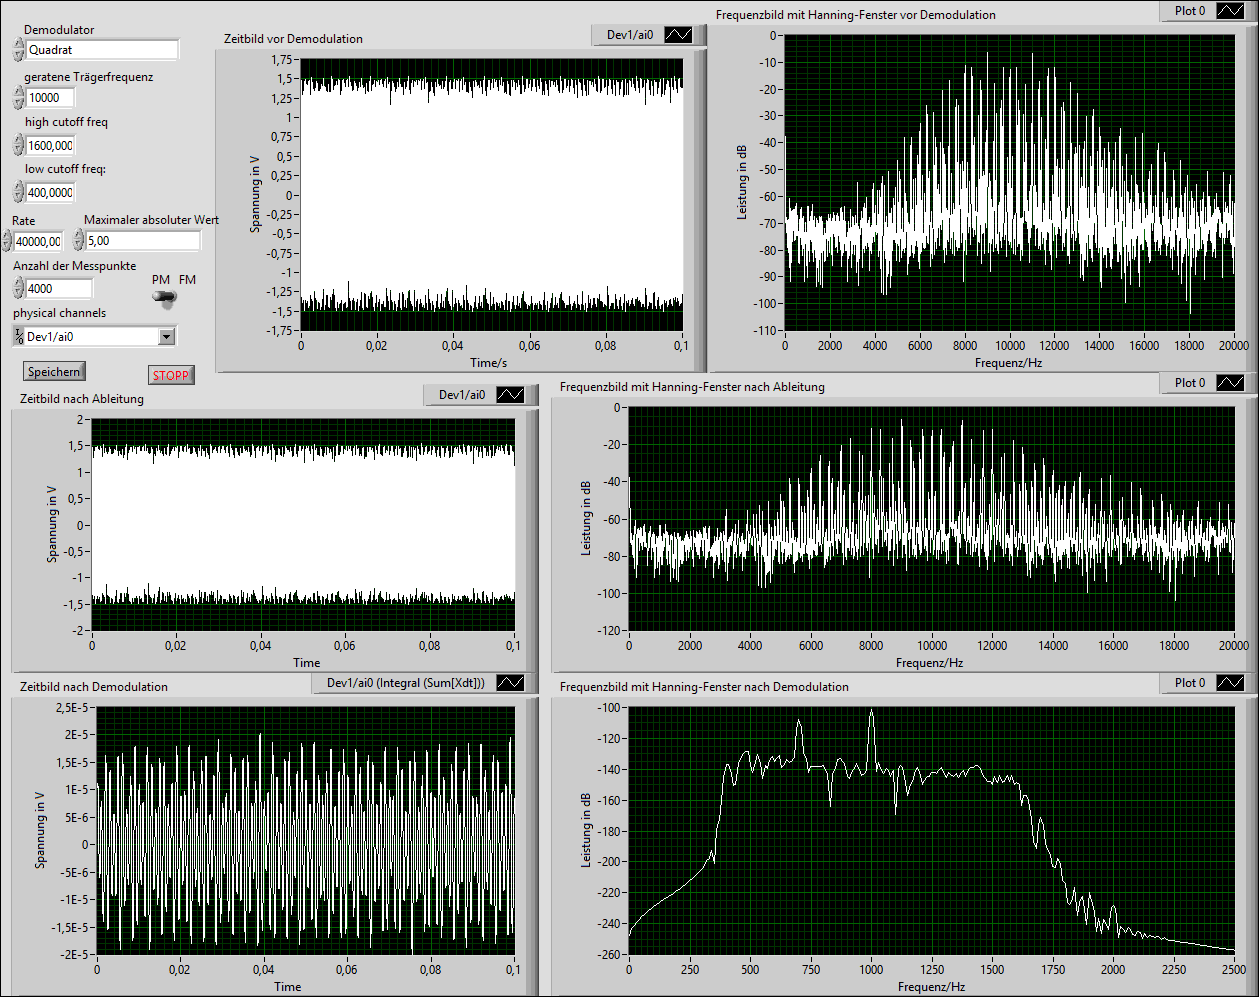
\includegraphics[width=1.0\textwidth]{EIRE2018Dateien/Tag4/OsziFMPM-Demod/mitBandpassUndIntegrationBilder/OsziPlusFMPMp}
		\caption{.}
	\end{figure}
\iffalse
	\begin{figure}[H] %FM-Diagramm mit Bandpass und Integration
		\centering
		\includegraphics[width=1.0\textwidth]{}
		\caption{.}
	\end{figure}

	\begin{figure}[H] %PM-Diagramm mit Bandpass und Integration 
		\centering
		\includegraphics[width=1.0\textwidth]{}
		\caption{.}
	\end{figure}
\fi
	
	%\printbibliography
\end{document}
